\part{Calculus (Single Variable)}
\chapter{Limits}
\section{Precise Definition of a Limit}
\begin{definition}
Let $f(x)$ be a function defined on an open interval around $x_0$. We say that the \vocab{limit} of $f(x)$ as $x$ approaches $x_0$ is $L$, that is $\displaystyle\lim_{x \to x_0}f(x)=L$, if for every $\epsilon>0$ there exists $\delta > 0$ such that $\forall x \in \RR$, 
\[ 0<\absolute{x-x_0}<\delta \implies \absolute{f(x)-L}<\epsilon \] 
\end{definition} 

Visualising this graphically, as $\epsilon$ becomes smaller and smaller, there always exists a $\delta$ that satisfies the property that for any $x$ in the open interval $(x_0-\delta,x_0+\delta)$, the value of $f(x)$ lies in the interval $(L-\epsilon, L+\epsilon)$.

\begin{figure}[H]
	\centering
	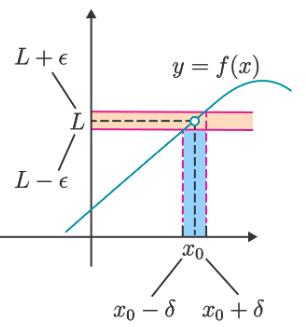
\includegraphics[width=0.3\linewidth]{images/Epsilon_delta_definition.png}
    \caption{Epsilon--delta definition}
\end{figure}

\begin{exercise} 
Prove that \[ \lim_{x\to3}2x+4=10. \]
\end{exercise}

Before the proof, we work backwards to find the value of $\delta$ in terms of $\epsilon$ and $x_0$, which we then declare in our proof.

$\forall \epsilon > 0$, $\exists \delta > 0$, $\forall x \in \RR$,
\[ |x-3| < \delta \implies |f(x)-10| < \epsilon \]
Let $\epsilon > 0$ be given.
\[ |f(x)-10| = |2x+4-10| = |2x-6| = 2|x-3| < \epsilon \]
Notice $|x-3| < \dfrac{\epsilon}{2}$. We can thus define $\delta \coloneqq \dfrac{\epsilon}{2}$. We now write our proof.

\begin{proof}
Let $\epsilon > 0$ be given. Choose $\delta = \dfrac{\epsilon}{2}$.

Then $\forall x \in \RR$, 
\begin{align*}
|x-3| &< \delta = \frac{\epsilon}{2} \\
2|x-3| &< \epsilon \\
|2x-6| &< \epsilon \\
|2x+4-10| &< \epsilon \\
|f(x)-10| &< \epsilon
\end{align*}
\end{proof}

\begin{exercise}
Use the formal definition of the limit to verify that 
\[ \lim_{x \to 3} \sqrt{2x+3} = 3. \]
\end{exercise}

We must prove that $\forall \epsilon > 0$, $\exists \delta > 0$ such that $\sqrt{2x+3} - 3 < \epsilon$ whenever $|x-3|<\delta$.
\begin{align*}
\sqrt{2x+3} - 3 &= \absolute{\frac{(2x+3)-3^2}{\sqrt{2x+3} + 3}} = \absolute{\frac{2x-6}{\sqrt{2x+3} + 3}} \\
&\le \absolute{\frac{2(x-3)}{3}} \\
&= \frac{2}{3} \absolute{x-3} < \frac{2}{3} \delta
\end{align*}
Hence, we can define 
\[ \epsilon \coloneqq \frac{2}{3} \delta \]
which we can use in our proof.

\begin{proposition}[Sum Law]
If $\lim_{x\to a}f(x)=L$ and $\lim_{x\to a}g(x)=M$ both exist, then
\[ \lim_{x\to a}[f(x)+g(x)]=L+M. \]
\end{proposition}

\begin{proof}
Let $\epsilon>0$ be given. We must find $\delta>0$ such that
\[ 0<|x-a|<\delta \implies |f(x)+g(x)-(L+M)|<\epsilon. \]
Using the Triangle Inequality we can write
\begin{align*}
\absolute{f(x)+g(x)-(L+M)}&=\absolute{\brac{f(x)-L}+\brac{g(x)-M}}\\
&\le|f(x)-L|+|g(x)-M|
\end{align*}
We make $\absolute{f(x)+g(x)-(L+M)}$ less than $\epsilon$ by making each of the terms $|f(x)-L|$ and $|g(x)-M|$ less than $\frac{\epsilon}{2}$.

Since $\frac{\epsilon}{2}>0$ and $\lim_{x\to a}f(x)=L$, there exists $\delta_1>0$ such that
\[ 0<|x-a|<\delta_1 \implies |f(x)-L|<\frac{\epsilon}{2}. \]
Similarly, since $\lim_{x\to a}g(x)=M$, there exists $\delta_2>0$ such that
\[ 0<|x-a|<\delta_2 \implies |g(x)-M|<\frac{\epsilon}{2}. \]
Let $\delta=\min\{\delta_1,\delta_2\}$, the smaller of the numbers $\delta_1$ and $\delta_2$. Notice that
\[ 0<|x-a|<\delta \implies 0<|x-a|<\delta_1 \text{ and } 0<|x-a|<\delta_2 \]
and so
\[ |f(x)-L|<\frac{\epsilon}{2} \text{ and } |g(x)-M|<\frac{\epsilon}{2}. \]
Therefore
\begin{align*}
\absolute{f(x)+g(x)-(L+M)}&\le|f(x)-L|+|g(x)-M|\\
&<\frac{\epsilon}{2}+\frac{\epsilon}{2}=\epsilon.
\end{align*}
To summarise,
\[ 0<|x-a|<\delta \implies \absolute{f(x)+g(x)-(L+M)}<\epsilon. \]
Thus by the definition of a limit,
\[ \lim_{x\to a}[f(x)+g(x)]=L+M. \]
\end{proof}
\pagebreak

\section{Limit Laws}
Let $f(x)$ and $g(x)$ be defined for all $x\neq a$ over some open interval containing $a$. Assume that $L$ and $M$ are real numbers such that $\lim_{x\to a}f(x)=L$ and $\lim_{x\to a}g(x)=M$, $c$ is a constant. Then each of the following statements holds.

\begin{itemize}
\item \textbf{Sum law}: The limit of a sum is the sum of the limits.
\[ \lim_{x\to a}(f(x)+g(x)) = \lim_{x\to a}f(x) + \lim_{x\to a}g(x) = L+M \]

\item \textbf{Difference law}: The limit of a difference is the difference of the limits.
\[ \lim_{x\to a}(f(x)-g(x)) = \lim_{x\to a}f(x) - \lim_{x\to a}g(x) = L-M \]

\item \textbf{Constant multiple law}: The limit of a constant times a function is the constant times the limit of the function.
\[ \lim_{x\to a}cf(x) = c\lim_{x\to a}f(x) = cL \]

\item \textbf{Product law}: The limit of a product is the product of the limits.
\[ \lim_{x\to a}(f(x)\cdot g(x)) = \lim_{x\to a}f(x) \cdot \lim_{x\to a}g(x) = L\cdot M \]

\item \textbf{Quotient law}: The limit of a quotient is the quotient of the limits.
\[ \lim_{x\to a}\frac{f(x)}{g(x)} = \frac{\lim_{x\to a}f(x)}{\lim_{x\to a}g(x)} = \frac{L}{M} \]
for $M \neq 0$.

\item \textbf{Power law}
\[ \lim_{x\to a}(f(x))^n = (\lim_{x\to a}f(x))^n = L^n \]
for every positive integer $n$.

\item \textbf{Root law}
\[ \lim_{x\to a}\sqrt[n]{f(x)} = \sqrt[n]{\lim_{x\to a}f(x)} = \sqrt[n]{L} \]
for all $L$ if $n$ is odd, and for $L\ge 0$ if $n$ is even.
\end{itemize}
\pagebreak

\section{Evaluating Limits}
Indeterminate forms of a limit include:
\[ \frac{0}{0} \quad \frac{\infty}{\infty} \quad 0 \times \infty \quad \infty - \infty \quad 0^0 \quad 1^{\infty} \quad \infty^0 \]
As long as limits are in indeterminate forms, they can still be evaluated.

Methods:
\begin{itemize}
\item Direct substitution

If $f$ is a polynomial or a rational function and $a$ is in the domain of $f$, then
\[ \lim_{x\to a}f(x)=f(a) \]

\item Cancel common factors
\item Multiply by the conjugate of the numerator or denominator
\end{itemize}

\begin{exercise}
Evaluate the following limit:
\[ \lim_{x\to 0} x^2\sin\brac{\frac{1}{x}} \]
\end{exercise}

\begin{solution}
If we plot the graph of the function out, we see that we can try to find two functions to apply Squeeze Theorem.

Notice that \[ -1 \le \sin\brac{\frac{1}{x}} \le 1 \]
and hence
\[ -x^2 \le x^2\sin\brac{\frac{1}{x}} \le x^2 \]
thus $x^2$ and $-x^2$ are the two functions that ``sandwich'' the given function.

Since $\lim_{x\to 0}x^2=0$ and $\lim_{x\to 0}-x^2=0$, applying Squeeze Theorem gives us 
\[ \lim_{x\to 0} x^2\sin\brac{\frac{1}{x}} = 0 \]
\end{solution}

\begin{exercise}
Evaluate the following limit:
\[ \lim_{x\to 3}\frac{-4x}{x-3} \]
\end{exercise}

\begin{solution}
Approaching from the left side,
\[ \lim_{x\to 3^-}\frac{-4x}{x-3} = +\infty \]
Approaching from the right side,
\[ \lim_{x\to 3^+}\frac{-4x}{x-3} = -\infty \]
Since $\lim_{x\to 3^-}\dfrac{-4x}{x-3} \neq \lim_{x\to 3^+}\dfrac{-4x}{x-3}$, the limit does not exist.
\end{solution}

\begin{theorem}
If $f(x) \le g(x)$ when $x$ is near $a$ (except possibly at $a$) and the limits of $f$ and $g$ both exist as $x$ approaches $a$, then
\[ \lim_{x\to a}f(x) \le \lim_{x\to a}g(x). \]
\end{theorem}

\begin{theorem}[Squeeze theorem]
Suppose that $g(x) \ge f(x) \ge h(x)$ for all $x$ in some open interval containing $c$ except possibly at $c$ itself. If $\lim_{x\to c} g(x) = L = \lim_{x\to c} h(x)$, then $\lim_{x\to c} f(x) = L$.
\end{theorem}

\begin{proof}
This can be proven using the epsilon--delta definition of limits.

Let $\epsilon > 0$ be given. We are done if we find a $\delta > 0$ such that $|f(x)-L| < \epsilon$ whenever $0 < |x-c| < \delta$.

Since $\lim_{x\to c} g(x) = L$, by definition of limits, there exists some $\delta_1 > 0$ such that for all $0 < |x-c| < \delta_1$, $|g(x)-L| < \epsilon$.
Thus, 
\[ -\epsilon < g(x)-L < \epsilon \quad \text{for all } 0 < |x-c| < \delta_1 \]
so
\begin{equation*}\tag{1}
L-\epsilon < g(x) < L + \epsilon \quad \text{for all } 0 < |x-c| < \delta_1
\end{equation*}
Similarly, since $\lim_{x\to c} h(x) = L$, by definition of limits, there exists some $\delta_2 > 0$ such that
\begin{equation*}\tag{2}
L-\epsilon < h(x) < L + \epsilon \quad \text{for all } 0 < |x-c| < \delta_2
\end{equation*}
Additionally, since $g(x) \le f(x) \le h(x)$ for all $x$ in some open interval containing $c$, there exists some $\delta_3 > 0$ such that for 
\begin{equation*}\tag{3}
g(x) \le f(x) \le h(x) \quad \text{for all } 0 < |x-c| < \delta_3
\end{equation*}
Now, we choose $\delta = \min(\delta_1, \delta_2, \delta_3)$. Then by (1), (3), and (2), we have 
\[ L-\epsilon < g(x) \le f(x) \le h(x) < L + \epsilon \quad \text{for all } 0 < |x-c| < \delta. \]
Therefore, $-\epsilon < f(x)-L < \epsilon$ for all $0 < |x-c| < \delta$, so
\[ |f(x)-L| < \epsilon \quad \text{for all } 0 < |x-c| < \delta. \]
Hence, by definition of limits, $\lim_{x\to c} f(x) = L$.
\end{proof}

\begin{theorem}[L'H\^{o}pital's Rule]
Let $f(x)$ and $g(x)$ be differentiable on an interval $I$ containing $c$, and that $g^\prime(c)\neq0$ on $I$ for $x \neq c$. Suppose that $\lim_{x\to c}\frac{f(x)}{g(x)}$ is in an indeterminate form. 

Then as long as the limits exist, we have 
\[ \lim_{x\to c}\frac{f(x)}{g(x)} = \lim_{x\to c}\frac{f^\prime(x)}{g^\prime(x)}. \]
\end{theorem}

\begin{proof}

\end{proof}

\begin{exercise}
Let $f$ be a differentiable function on $(0,\infty)$ and suppose that $\lim_{x\to\infty}\brac{f(x)+f^\prime(x)}=L$.

By considering $f(x)=\dfrac{e^xf(x)}{e^x}$, show that $\lim_{x\to\infty}f(x)=L$ and $\lim_{x\to\infty}f^\prime(x)=0$.
\end{exercise}

\begin{solution}
We may apply L'H\^{o}pital's Rule as we encounter $\dfrac{\infty}{\infty}$ in $\displaystyle\lim_{x\to\infty}\frac{e^xf(x)}{e^x}$.

\[ \lim_{x\to\infty}f(x)=\lim_{x\to\infty}\frac{e^xf(x)}{e^x}=\lim_{x\to\infty}\frac{\brac{e^xf(x)}^\prime}{\brac{e^x}^\prime}=\lim_{x\to\infty}\frac{e^xf(x)+e^xf^\prime(x)}{e^x}=L \]

Hence $\lim_{x\to\infty}f(x)=L$ and $\lim_{x\to\infty}f^\prime(x)=0$.
\end{solution}
\pagebreak

% uniqueness of the limit


\section{Important Limits}
\begin{equation}
\lim_{x \to 0} \frac{\sin x}{x} = 1
\end{equation}
\begin{proof}
This can be proven using the squeeze theorem, which will be discussed later.
\end{proof}

\begin{equation}
\lim_{x \to 0} \frac{1-\cos x}{x} = 0
\end{equation}
\begin{proof}
This can be proven using the squeeze theorem, which will be discussed later.
\end{proof}

\begin{equation}
\lim_{x\to 0} \frac{\arcsin x}{x} = 1
\end{equation}

\begin{equation}
\lim_{x\to \pm\infty} \brac{1+\frac{1}{x}}^x=e
\end{equation}
\pagebreak

\section{Continuity}
\begin{definition}
A function $f(x)$ is \vocab{continuous} at $x=a$ if 
\[ \lim_{x\to a} f(x)=f(a). \]
A function is said to be continuous on the interval $[a,b]$ if it is continuous at each point in the interval.
\end{definition}

Note that this definition is also implicitly assuming that both $f(a)$ and $\lim_{x\to a}f(x)$ exist. If either of these do not exist the function will not be continuous at $x=a$.

This definition can be turned around into the following fact.
\begin{corollary}
If $f(x)$ is continuous at $x=a$ then
\[ \lim_{x \to a} f(x) = f(a) \quad \lim_{x \to a^-} f(x) = f(a) \quad \lim_{x \to a^+} f(x) = f(a) \]
\end{corollary}

A nice consequence of continuity is the following fact.
\begin{corollary}
If $f(x)$ is continuous at $x=b$ and $\lim_{x\to a}g(x)=b$ then
\[ \lim_{x \to a} f(g(x)) = f\brac{\lim_{x \to a} g(x)} \]
\end{corollary}

\begin{exercise}
Evaluate the following limit:
\[ \lim_{x \to 0} e^{\sin x} \]
\end{exercise}

\begin{solution}
Since we know that exponentials are continuous everywhere we can use the fact above.
\[ \lim_{x \to 0} e^{\sin x} = e^{\lim_{x \to 0} \sin x} = e^0 = \boxed{1} \]
\end{solution}

Another very nice consequence of continuity is the Intermediate Value Theorem.
\begin{theorem}[Intermediate Value Theorem]
Suppose that $f(x)$ is continuous on $[a,b]$ and let $M$ be any number between $f(a)$ and $f(b)$. Then there exists $c \in (a,b)$ such that $f(c)=M$.
\end{theorem}
All the Intermediate Value Theorem is really saying is that a continuous function will take on all values between $f(a)$ and $f(b)$.
\pagebreak

\chapter{Derivative}
\section{Definitions}
\begin{definition}
The \vocab{derivative} of $f(x)$ with respect to $x$, denoted by $f^\prime(x)$, is defined as 
\begin{equation} f^\prime (x) = \lim_{h \to 0} \frac{f(x+h)-f(x)}{h}.
\end{equation}
\end{definition}

The right-hand derivative of $f(x)$ at $x=x_0$ is defined as
\[ f_+^\prime(x_0)=\lim_{h\to0^+}\frac{f(x_0+h)-f(x_0)}{h}. \]
Similarly, the left-hand derivative of $f(x)$ at $x=x_0$ is defined as
\[ f_-^\prime(x_0)=\lim_{h\to0^-}\frac{f(x_0+h)-f(x_0)}{h}. \]
A function $f$ has a derivative at $x=x_0$ if and only if $f_+^\prime(x_0)=f_-^\prime(x_0)$.

\begin{definition} 
$f(x)$ is \vocab{differentiable} at $x_0$ if $f^\prime(x_0)$ exists; $f(x)$ is differentiable on an interval $I$ if the derivative exists for every $x\in I$.
\end{definition}

\begin{theorem}
$f(x)$ is continuous at $x_0$ if $f(x)$ is differentiable at $x=x_0$.
\end{theorem}

\begin{proof}
To prove that $f$ is continuous at $x_0$, we have to show that $\lim_{x\to x_0}f(x)=f(x_0)$. We will do this by showing that the difference $f(x)-f(x_0)$ approaches $0$.

Given that $f$ is differentiable at $x_0$,
\[ f^\prime(x_0)=\lim_{x\to x_0}\frac{f(x)-f(x_0)}{x-x_0} \]
exists. We can rewrite
\[ f(x)-f(x_0)=\frac{f(x)-f(x_0)}{x-x_0}(x-x_0). \]
Then
\begin{align*}
\lim_{x\to x_0}[f(x)-f(x_0)]
&=\lim_{x\to x_0}\frac{f(x)-f(x_0)}{x-x_0}(x-x_0)\\
&=\lim_{x\to x_0}\frac{f(x)-f(x_0)}{x-x_0}\cdot\lim_{x\to x_0}(x-x_0)\\
&=f^\prime(x_0)\cdot0=0
\end{align*}
To use what we have just proved, 
\begin{align*}
\lim_{x\to x_0}f(x)
&=\lim_{x\to x_0}[f(x_0)+\brac{f(x)-f(x_0)}]\\
&=\lim_{x\to x_0}f(x_0)+\lim_{x\to x_0}[f(x)-f(x_0)]\\
&=f(x_0)+0=f(x_0)
\end{align*}
Therefore $f$ is continuous at $x_0$.
\end{proof}

\begin{remark}
This means differentiability implies continuity. However the converse is not necessarily true, one notable example being the Weierstrass function.
\end{remark}
\pagebreak

\section{Theorems}
\begin{definition}
Let $c$ be a number in the domain $D_f$ of a function $f$. Then $f(c)$ is the
\begin{itemize}
\item \vocab{absolute maximum} value of $f$ on $D_f$ if $f(c)\ge f(x)$ for all $x\in D_f$.
\item \vocab{absolute minimum} value of $f$ on $D_f$ if $f(c)\le f(x)$ for all $x\in D_f$.
\end{itemize}
\end{definition}

An absolute maximum or minimum is sometimes called a \emph{global} maximum or minimum. The maximum and minimum values of $f$ are called \vocab{extreme values} of $f$.

\begin{definition}
$f(c)$ is a
\begin{itemize}
\item \vocab{local maximum} value of $f$ if $f(c)\ge f(x)$ when $x$ is near $c$.
\item \vocab{local minimum} value of $f$ if $f(c)\le f(x)$ when $x$ is near $c$.
\end{itemize}
\end{definition}

We have seen that some functions have extreme values, whereas others do not. The following theorem gives conditions under which a function is guaranteed to possess extreme values.

\begin{theorem}[Extreme Value Theorem]
For a function $f$ continuous on $[a,b]$, it attains its maximum and minimum values on $[a,b]$.
\end{theorem}

\begin{proof}
We prove the case that $f$ attains its maximum value on $[a,b]$.

Since $f$ is continuous on $[a,b]$, we know it must be bounded on $[a,b]$ by the Boundedness Theorem. Let $M = \sup f$.

If there is some $c \in [a,b]$ where $f(c)=M$ there is nothing more to show -- $f$ attains its maximum on $[a,b]$.

Suppose otherwise, that there is no such $c$. Then $f(x)<M$ for all $x \in [a,b]$.

We define a new function $g$ by 
\[ g(x) = \frac{1}{M-f(x)}. \]

Note that $g(x)>0$ for every $x \in [a,b]$ and $g$ is continuous on $[a,b]$, and thus also bounded on this interval, again by the Boundedness theorem.

Given that $g$ is bounded on $[a,b]$, there must exist some $K>0$ such that $g(x) \le K$ for every $x \in [a,b]$.

Consequently,
\[ \frac{1}{M-f(x)} \le K \implies f(x) \le M - \frac{1}{K} \]
for every $x \in [a,b]$. This contradicts the assumption that $M$ is the least upper bound.

That leaves as the only possibility that there is some $c$ in $[a,b]$ where $f(c)=M$. That is to say, $f$ attains its maximum on $[a,b]$.

The proof that $f$ attains its minimum on the same interval is argued similarly and is left as an exercise for the reader.
\end{proof}

\begin{theorem}[Fermat's Theorem]
If $f$ has a local maximum or minimum at $c$, and if $f^\prime(c)$ exists, then $f^\prime(c)=0$.
\end{theorem}

\begin{proof}
Suppose, for the sake of definiteness, that $f$ has a local maximum at $c$. Then $f(c)\ge f(x)$ if $x$ is sufficiently close to $c$. This implies that if $h$ is sufficiently close to $0$, with $h$ being positive or negative, then
\[ f(c)\ge f(c+h) \]
and thus
\[ f(c+h)-f(c)\le0. \]
We can divide both sides of an inequality by a positive number. Thus, if $h>0$ and $h$ is sufficiently small, we have
\[ \frac{f(c+h)-f(c)}{h}\le0. \]
Taking the right-hand limit of both sides of the inequality,
\[ \lim_{h\to0^+}\frac{f(c+h)-f(c)}{h}\le\lim_{h\to0^+}0=0 \]
but since $f^\prime(c)$ exists, we have
\[ f^\prime(c)=\lim_{h\to0}\frac{f(c+h)-f(c)}{h}=\lim_{h\to0^+}\frac{f(c+h)-f(c)}{h} \]
and so we have show that $f^\prime(c)\le0$.

On the other hand, if $h<0$, then the direction of the inequality is reversed when we divide by $h$:
\[ \frac{f(c+h)-f(c)}{h}\ge0 \]
so taking the left-hand limit, we have
\[ f^\prime(c)=\lim_{h\to0}\frac{f(c+h)-f(c)}{h}=\lim_{h\to0-}\frac{f(c+h)-f(c)}{h}\ge0 \]
thus $f^\prime(c)\ge0$.

Since $f^\prime(c)\ge0$ and $f^\prime(c)\le0$, we have $f^\prime(c)=0$.

We have proved Fermat's Theorem for the case of a local maximum. The case of a local minimum can be proved in a similar manner.
\end{proof}

\begin{theorem}[Rolle's Theorem]
Let $f:[a,b]\to\RR$ be continuous on $[a,b]$ and differentiable on $(a,b)$, and $f(a)=f(b)$. Then there exists $c \in (a,b)$ such that 
\[ f^\prime(c)=0. \]
\end{theorem}
\begin{remark}
Rolle's Theorem is simply a special case of the Mean Value Theorem, where $f(a)=f(b)$.
\end{remark}

\begin{proof}
\textbf{Case 1:} $f(x)=k$ where $k$ is a constant

Then $f^\prime(x)=0$, so the number $c$ can be taken to be any number in $(a,b)$.

\textbf{Case 2:} $f(x)>f(a)$ for some $x\in(a,b)$

By the Extreme Value Theorem, $f$ has a maximum value somewhere in $[a,b]$. Since $f(a)=f(b)$, it must attain this maximum value at a number $c$ in the open interval $(a,b)$. Then $f$ has a local maximum at $c$, thus $f$ is differentiable at $c$. Therefore $f^\prime(c)=0$ by Fermat's Theorem.

\textbf{Case 3:} $f(x)<f(a)$ for some $x\in(a,b)$

By the Extreme Value Theorem, $f$ has a minimum value in $[a,b]$ and, since $f(a)=f(b)$, it attains this minimum value at a number $c\in(a,b)$. Again $f^\prime(c)=0$ by Fermat's Theorem.
\end{proof}

\begin{theorem}[Mean Value Theorem]
Let $f:[a,b]\to\RR$ be continuous on $[a,b]$ and differentiable on $(a,b)$. Then there exists $c\in(a,b)$ such that 
\[ f^\prime(c)=\frac{f(b)-f(a)}{b-a}. \]
\end{theorem}

\begin{figure}[H]
    \centering
    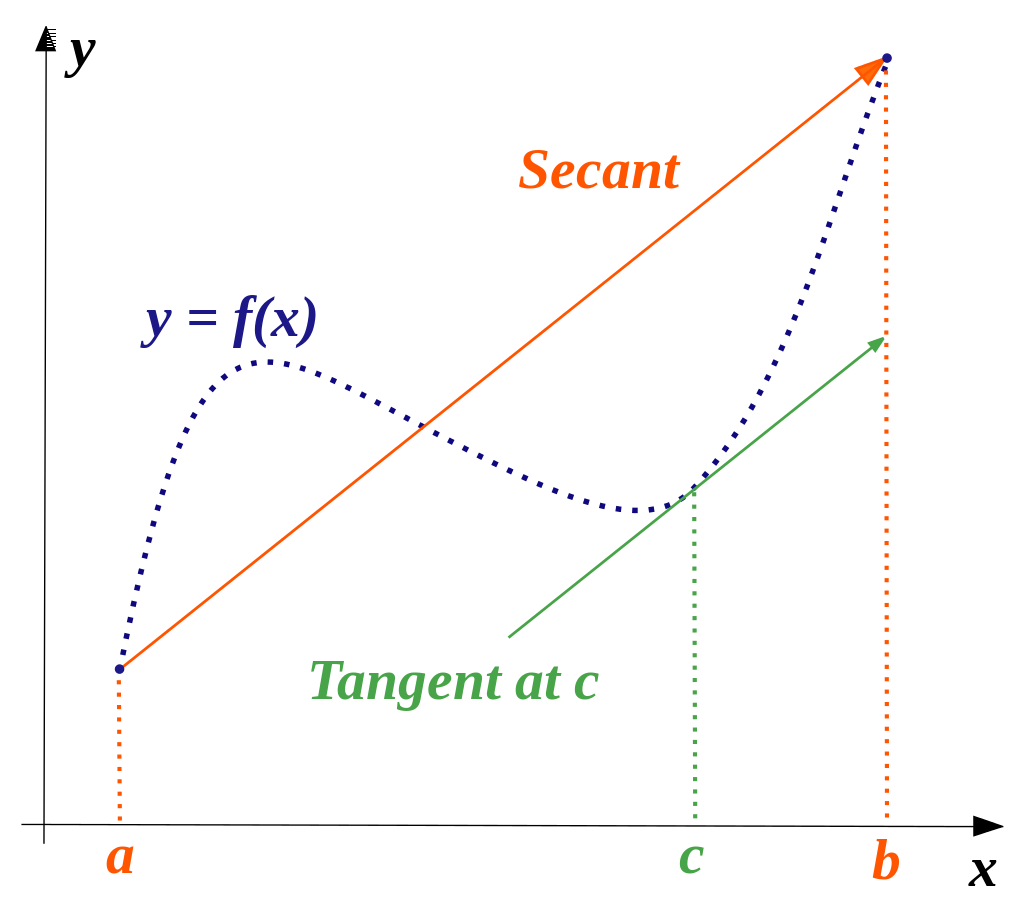
\includegraphics[width=8cm]{images/mean_value_thrm.png}
    \caption{Mean value theorem}
\end{figure}

\begin{theorem}[Cauchy's Generalised Theorem of the Mean]
Let $f$ and $g$ be continuous on $[a,b]$ and differentiable on $(a,b)$, and where $g(x)\neq0$ in $(a,b)$. Then there exists $c\in(a,b)$ such that
\[ \frac{f^\prime(c)}{g^\prime(c)}=\frac{f(b)-f(a)}{g(b)-g(a)}. \]
\end{theorem}

In layman's term, the theorem states that given two differentiable functions, there is some point $c$ where the ratio of their average rates of change agrees with the ratio of their instantaneous rates of change.

\begin{remark}
When $g(x)=x$, it reduces to the Mean Value Theorem.
\end{remark}

\begin{exercise}
Let $f(x)=\dfrac{x^e}{e^x}$, where $x>0$. Find the maximum value of $f(x)$ and hence prove that $e^\pi>\pi^e$.
\end{exercise}

\begin{proof}
\[ f^\prime(x)=x^{e-1}e^{-x}(e-x) \]
Since $x^{e-1}e^{-x}>0$ for all $x>0$, we have
\[ f^\prime(x)=\begin{cases}
>0 & x<e\\
0 & x=e\\
<0 & x>e
\end{cases}. \]
Hence the maximum value of $f$ occurs at $x=e$ since $f$ is a continuous function, with maximum value $f(e)=\dfrac{e^e}{e^e}=1$.

Therefore $\dfrac{x^e}{e^x}<1$ for all $x\in\RR^+\setminus\{e\}$, i.e. $\dfrac{\pi^e}{e^\pi}<1$ and thus $e^\pi>\pi^e$.
\end{proof}

\begin{exercise}
By applying Rolle's Theorem on the function $f(x)=e^{-x}-\sin x$, show that there is at least one real root of $e^x\cos x=-1$ between any two real roots of $e^x\sin x=1$.
\end{exercise}

\begin{proof}
Let the two real roots involved of $e^x\sin x=1$ be $a$ and $b$ with $a<b$.

Then $f(a)=f(b)=0$. By Rolle's Theorem, there exist a value $c$ with $a<c<b$ such that $f^\prime(c)=0$, i.e. $-e^{-c}-\cos c=0$ which reduces to $e^c\cos c=-1$.
\end{proof}

\begin{exercise}
By using the Theorem of the Mean, show that
\[ \frac{\pi}{6}+\frac{\sqrt{3}}{15}<\sin^{-1}0.6<\frac{\pi}{6}+\frac{1}{8}. \]
\end{exercise}

\begin{proof}
Let $f(x)=\sin^{-1}x$, we have $f^\prime(x)=\dfrac{1}{\sqrt{1-x^2}}$.

By the Theorem of the Mean, we have, for $a<c<b$,
\[ \frac{1}{\sqrt{1-a^2}}<\frac{1}{\sqrt{1-c^2}}=\frac{\sin^{-1}(b)-\sin^{-1}(a)}{b-a}<\frac{1}{\sqrt{1-b^2}}. \]
i.e. Interval min grad / Interval average grad/ Interval max grad

Using $a=0.5$ and $b=0.6$,
\begin{align*}
&\frac{1}{\sqrt{1-0.5^2}}<\frac{\sin^{-1}0.6-\sin^{-1}0.5}{0.6-0.5}<\frac{1}{\sqrt{1-0.6^2}} \\
&\frac{2}{\sqrt{3}}<\frac{\sin^{-1}0.6-\frac{\pi}{6}}{0.1}<\frac{1}{0.8} \\
&\frac{\sqrt{3}}{15}<\sin^{-1}0.6-\frac{\pi}{6}<\frac{1}{8} \\
&\frac{\pi}{6}+\frac{\sqrt{3}}{15}<\sin^{-1}0.6<\frac{\pi}{6}+\frac{1}{8}
\end{align*}
\end{proof}
\pagebreak

\section{Differentiation Rules}
For a constant $c\in\RR$ and functions $f$ and $g$ of $x$, the following rules hold.

\begin{itemize}
\item \textbf{Scalar multiplication}
\[ (cf)^\prime = cf^\prime \]

\item \textbf{Addition rule}
\[ (f+g)^\prime = f^\prime + g^\prime \]

\begin{proof}
\begin{align*}
(f + g)^\prime (x) &= \lim_{h \to 0} \frac{(f+g)(x+h) - (f+g)(x)}{h}\\
&= \lim_{h \to 0} \frac{f(x+h) + g(x+h) - f(x) - g(x)}{h}\\
&= \lim_{h \to 0} \left[ \frac{f(x+h) - f(x)}{h} + \frac{g(x+h) - g(x)}{h} \right] \\
&= \lim_{h \to 0} \frac{f(x+h) - f(x)}{h} + \lim_{h \to 0} \frac{g(x+h) - g(x)}{h}\\
&= f^\prime (x) + g^\prime (x)
\end{align*}
\end{proof}

\item \textbf{Power rule}
\[ \dv{x} x^n = n x^{n-1} \]

\begin{proof}
Using implicit differentiation,
\begin{align*}
y &= x^n \\
\ln y &= \ln x^n \\
\ln y &= n \ln x \\
\frac{y^\prime}{y} &= n \frac{1}{x}
\end{align*}
\[ y^\prime = y \frac{n}{x} = x^n \brac{\frac{n}{x}} = n x^{n-1} \]
\end{proof}

\item \textbf{Product rule}
\[ (fg)^\prime = f^\prime g + f g^\prime \]

\begin{proof}
\begin{align*}
(fg)^\prime (x) &= \lim_{h \to 0} \frac{(fg)(x+h) - (fg)(x)}{h}\\
&= \lim_{h \to 0} \frac{f(x+h) g(x+h) - f(x) g(x)}{h}\\
&= \lim_{h \to 0} \frac{f(x+h) g(x) - f(x) g(x) + f(x+h) g(x+h) - f(x+h) g(x)}{h}\\
&= \lim_{h \to 0} \frac{f(x+h) g(x) - f(x) g(x)}{h} + \lim_{h \to 0} \frac{f(x+h) g(x+h) - f(x+h) g(x)}{h}\\
&= \lim_{h \to 0} \frac{f(x+h) - f(x)}{h}g(x) + \lim_{h \to 0} \frac{g(x+h) - g(x)}{h}f(x+h)\\
&= \left[\lim_{h \to 0} \frac{f(x+h) - f(x)}{h}\right] g(x) + \left[\lim_{h \to 0} \frac{g(x+h) - g(x)}{h}\right] f(x)\\
&= f^\prime (x) g(x) + f(x) g^\prime (x)
\end{align*}
\end{proof}

\item \textbf{Quotient rule}
\[ \brac{\frac{f}{g}}^\prime = \frac{f^\prime g - fg^\prime}{g^2} \] 

\begin{proof}
\begin{align*}
\left[\frac{f(x)}{g(x)}\right]^\prime &= \lim_{h \to 0} \frac{\frac{f(x+h)}{g(x+h)} - \frac{f(x)}{g(x)}}{h}\\
&= \lim_{h \to 0} \frac{1}{h} \frac{f(x+h) g(x) - f(x) g(x+h)}{g(x+h) g(x)}\\
&= \lim_{h \to 0} \frac{1}{h} \frac{f(x+h) g(x) - f(x) g(x) + f(x) g(x) - f(x) g(x+h)}{g(x+h) g(x)}\\
&= \lim_{h \to 0} \frac{1}{g(x+h) g(x)} \left[ \frac{f(x+h)g(x) - f(x)g(x)}{h} + \frac{f(x)g(x) - f(x)g(x+h)}{h} \right] \\
&= \lim_{h \to 0} \frac{1}{g(x+h) g(x)} \left[ g(x)\frac{f(x+h) - f(x)}{h} - f(x)\frac{g(x) + g(x+h)}{h} \right] \\
&= \frac{1}{g^2(x)} [g(x) f^\prime(x) - f(x) g^\prime(x)] \\
&= \frac{f^\prime(x) g(x) - f(x) g^\prime(x)}{g^2(x)}
\end{align*}
\end{proof}

\item \textbf{Chain rule}
\begin{theorem}[Chain rule] 
If $f$ and $g$ are both differentiable functions and we define $F(x)=(f\circ g)(x)$, then the derivative of $F(x)$ is
\begin{equation}
F^\prime (x) = f^\prime(g(x)) g^\prime(x) 
\end{equation}
\end{theorem}
\end{itemize}

\section{Applications of Differentiation}
\subsection{Implicit differentiation}
\textbf{Implicit differentiation} simply means differentiating both sides of the equation with respect to a variable.

\subsection{Newton's Method}
In this section we are going to look at a method for approximating solutions to equations.

\begin{figure}[H]
    \centering
    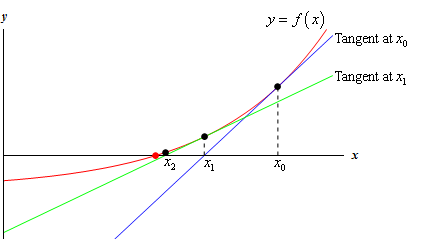
\includegraphics[width=10cm]{images/newton_method.png}
\end{figure}

Suppose that we want to approximate the solution to $f(x)=0$. Suppose that we have somehow found an initial rough approximation to the solution: $x=x_0$. The tangent line to $f(x)$ at $x=x_0$ is
\[ y = f(x_0) + f^\prime(x_0)(x-x_0) \]

This tangent line crosses the $x$-axis much closer to the actual solution to the equation than $x_0$ does. Let the tangent at $x_0$ intersect $x$-axis at $x_1$. We use this point as our new approximation to the solution. $x_1$ is given by:
\[ x_1 = x_0 - \frac{f(x_0)}{f^\prime(x_0)} \]

Repeat the process; form up the tangent line at $x_1$ and use its root $x_2$ as a new approximation:
\[ x_2 = x_1 - \frac{f(x_1)}{f^\prime(x_1)} \]

Here is the general Newton's Method:
\begin{theorem}[Newton's Method]
If $x_n$ is an approximation of a solution of $f(x)=0$ and if $f^\prime(x_n) \neq 0$, then the next approximation is given by
\[ x_{n+1} = x_n - \frac{f(x_n)}{f^\prime(x_n)} \]
\end{theorem}
\pagebreak

\chapter{Integral}
\section{Definition}
We use the \textbf{Riemann} definition of an integral:
\begin{definition}
An \vocab{integral} is defined as an infinite sum over an interval.
\begin{equation}
\int_a^b f(x) \dd{x} = \lim_{n \to \infty} \sum_{i=1}^n f(x_i) \Delta x
\end{equation}
\end{definition}

A Riemann sum is an approximation of an integral by a finite sum.

Let $f$ be defined on the closed interval $[a,b]$ and let $\Delta x$ be a partition of $[a,b]$, with
\[ a=x_1 < x_2 < \cdots < x_n < x_{n+1}=b.\]

Let $\Delta x_i$ denote the length of the $i$th subinterval $[x_i,x_{i+1}]$ and let $c_i$ denote any value in the $i$th subinterval.

The sum
\[ \sum_{i=1}^n f(c_i)\Delta x_i\]
is a Riemann sum of $f$ on $[a,b]$.

As the subinterval becomes infinitesimally small, 
\[ \int _{a}^{b}f(x) \dd{x} = \lim _{\Delta x \to 0} \sum _{i=1}^{n} f(x_{i}) \Delta x_{i} \]

\begin{figure}[H]
	\centering
	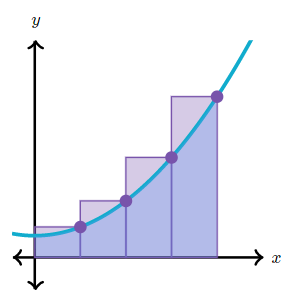
\includegraphics[width=8cm]{Riemanns_sums}
\end{figure}

\begin{theorem}[Fundamental Theorem of Calculus]
The fundamental theorem of (single variable) calculus states that if $f^\prime$ is continuous on $[a,b]$, then the integral of the derivative across the bounds is equal to the original function at the bounds:
\begin{equation}
\int_a^b f^\prime(x) \dd{x} = f(b)-f(a)
\end{equation}
or equivalently,
\begin{equation}
\dv{x} \int_{a}^{x} f(s) \dd{s} = f(x)
\end{equation}
\end{theorem}

% https://www2.clarku.edu/faculty/djoyce/ma121/FTCproof.pdf

Using the definition of the derivative, we differentiate the following integral:
\begin{align*}
\dv{x} \int_{a}^{x} f(s) \dd{s} &= \lim_{h \to 0} \frac{\int_{a}^{x+h} f(s) \dd{s} - \int_{a}^{x} f(s) \dd{s}}{h}\\
&= \lim_{h \to 0} \frac{\int_{x}^{x+h} f(s) \dd{s}}{h}\\
&= \lim_{h \to 0} \frac{h f(x)}{h}\\
&= f(x)
\end{align*}
% https://math.libretexts.org/Bookshelves/Calculus/Calculus_3e_(Apex)/05%3A_Integration/5.04%3A_The_Fundamental_Theorem_of_Calculus

\section{Integration Rules}
For constant $k\in\RR$ and functions $f(x)$ and $g(x)$, the following rules hold.
\begin{itemize}
\item \textbf{Sum and difference rule}
\[ \int f(x)\pm g(x) \dd{x} = \int f(x) \dd{x} \pm \int g(x) \dd{x} \]

\item \textbf{Scalar multiplication}
\[ \int kf(x) \dd{x} = k\int f(x) \dd{x} \]

\item \textbf{Power rule}
\[ \int x^n \dd{x} = \frac{x^{n+1}}{n+1} + C \]

\item \textbf{Constant rule}
\[ \int a\dd{x} = ax + C \]
\end{itemize}

\section{Integration Techniques}
\subsubsection{Integrals of powers and of trigonometric functions}
Reciprocal rules:
\[ \int \frac{1}{x} \dd{x} = \ln|x| + C \]
\[ \int \frac{1}{ax+b} \dd{x} = \frac{1}{a} \ln(ax+b) + C \]

Exponential functions:
\[ \int e^x \dd{x} = e^x + C \]
\[ \int a^{x} \dd{x} = \frac{a^x}{\ln a} + C \]

Natural log rule:
\[ \int \ln x \dd{x} = x\ln x - x + C \]

Trigonometric functions:
\[ \int \sin x \dd{x} = -\cos x + C \]

\[ \int \cos x \dd{x} = \sin x + C \]

\[ \int \tan x \dd{x} = \ln|\sec x| + C \]

\[ \int \cosec x \dd{x} = \ln|\cosec x - \cot x| + C \]

\[ \int \cosec^2x \dd{x} = -\cot x + C \]

\[ \cosec x \cot x \dd{x} = -\cosec x + C \]

\[ \sec x \dd{x} = \ln|\sec x + \tan x| + C \]

\[ \int \sec^2 x \dd{x} = \tan x + C \]

\[ \int \sec x \tan x \dd{x} = \sec x + C \]

\[ \int \cot x \dd{x} = \ln|\sin x| + C \]

Inverse trigonometric functions:
\[ \int\frac{1}{\sqrt{1-x^2}}\dd{x} = \sin^{-1}x + C \]
\[ \int-\frac{1}{\sqrt{1-x^2}}\dd{x} = \cos^{-1}x + C \]
\[ \int\frac{x}{1+x^2}\dd{x} = \tan^{-1}x + C \]

\subsubsection{Splitting the Numerator}
\begin{exercise}
Evaluate exactly
\[ \int_0^1\frac{x+2}{\sqrt{x+1}}\dd{x}. \]
\end{exercise}
\begin{solution}
\begin{align*}
\int_0^1\frac{x+2}{\sqrt{x+1}}\dd{x}
&= \int_0^1\brac{\sqrt{x+1}+\frac{1}{\sqrt{x+1}}}\dd{x} \\
&= \sqbrac{\frac{2}{3}(x+1)^\frac{3}{2}+2(x+1)^\frac{1}{2}}_0^1 \\
&= \boxed{\frac{2}{3}\brac{5\sqrt{3}-4}}
\end{align*}
\end{solution}

\subsubsection{Substitution}
\begin{equation}
\int f(g(x)) g^\prime (x)\dd{x} = \int f(u) \dd{u}
\end{equation}
where $u=g(x)$.

The most common way of doing a integral by substitution, and the only way for indefinite integrals, is as follows:
\begin{enumerate}
\item Change variables from $x$ to $u$ (hence the common name ``$u$-substitution'')
\item Keep track of the relation between $\dd{x}$ and $\dd{u}$
\item If you chose correctly you can now do the $u$-integral
\item When you are done, substitute back for $x$
\end{enumerate}

\begin{exercise}
Compute $\int\sin^nx\cos x\dd{x}$.
\end{exercise}
\begin{solution}
Substitute $u = \sin x$ and $\dd{u} = \cos x\dd{x}$. This turns the integral into $\int u^n\dd{u}$ which is easily valuated as $u^{n+1}/(n+1)$. Now plug back in $u = \sin x$ and you get the answer
\[ \frac{\sin^{n+1}x}{n+1}. \]
\end{solution}

\begin{exercise}
Compute $\displaystyle\int_1^2\frac{x}{x^2+1}\dd{x}$.
\end{exercise}
\begin{solution}
Let $u=x^2+1$ then $\dd{u} = 2x\dd{x}$, so the integrand becomes $(1/2)\dd{u}/u$. If $x$ goes
from 1 to 2 then $u$ goes from 2 to 5, thus the integral becomes
\[ \int_2^5\frac{1}{2}\frac{\dd{u}}{u} = \frac{1}{2}(\ln5-\ln2). \]
\end{solution}

\begin{exercise}
Compute $\int xe^{x^2}\dd{x}$.
\end{exercise}
\begin{solution}
To do this integral we'll use the following substitution.
\[ u=x^2 \implies \dd{u}=2x\dd{x} \implies x\dd{x}=\frac{1}{2}\dd{u} \]
\[ \int x e^{x^2}\dd{x} = \frac{1}{2}\int e^u \dd{u} = \frac{1}{2}e^u + c = \frac{1}{2}e^{x^2} + c \]
\end{solution}

\begin{exercise}
Prove the following result for $a>0$:
\begin{equation*}\tag{*}
\int_0^af(x)\dd{x}=\int_0^af(a-x)\dd{x}
\end{equation*}
Hence evaluate
\begin{enumerate}[label=(\alph*)]
\item $\displaystyle\int_0^\frac{\pi}{2}\frac{\cos^nx}{\sin^nx+\cos^nx}\dd{x}$, where $n$ is a real constant,
\item $\displaystyle\int_0^a\frac{x^4}{x^4+(x-a)^4}\dd{x}$, where $a$ is a positive real constant.
\end{enumerate}
\end{exercise}
\begin{solution}
Substitute $x=a-u\implies\dv{x}{u}=-1$.

For the lower and upper limits, $x=0\implies u=a$ and $x=a\implies u=0$ respectively.

Using the substitution, we have
\[ \int_0^af(x)\dd{x}=\int_a^0f(a-u)(-1)\dd{u}=\int_0^af(a-u)\dd{u}=\int_0^af(a-x)\dd{x}. \]

\begin{enumerate}[label=(\alph*)]
\item For $f(x)=\dfrac{\cos^nx}{\sin^nx+\cos^nx}$ with $a=\frac{\pi}{2}$,
\[ f\brac{\frac{\pi}{2}-x}=\frac{\cos^n\brac{\frac{\pi}{2}-x}}{\sin^n\brac{\frac{\pi}{2}-x}+\cos^n\brac{\frac{\pi}{2}-x}}=\frac{\sin^nx}{\cos^nx+\sin^nx}. \]
By (*), 
\[ \int_0^\frac{\pi}{2}f(x)\dd{x}=\int_0^\frac{\pi}{2}f\brac{\frac{\pi}{2}-x}\dd{x} \]
So we have
\[ \int_0^\frac{\pi}{2}\frac{\cos^nx}{\sin^nx+\cos^nx}\dd{x}=\int_0^\frac{\pi}{2}\frac{\sin^nx}{\sin^nx+\cos^nx}\dd{x} \]
Let $\displaystyle I=\int_0^\frac{\pi}{2}\frac{\cos^nx}{\sin^nx+\cos^nx}\dd{x}=\int_0^\frac{\pi}{2}\frac{\sin^nx}{\sin^nx+\cos^nx}\dd{x}$.

Then
\[ 2I=I+I=\int_0^\frac{\pi}{2}\frac{\sin^nx+\cos^nx}{\sin^nx+\cos^nx}\dd{x}=\int_0^\frac{\pi}{2}1\dd{x}=\frac{\pi}{2} \]
Hence $\displaystyle I=\int_0^\frac{\pi}{2}\frac{\cos^nx}{\sin^nx+\cos^nx}\dd{x}=\boxed{\frac{\pi}{4}}$

\item Let $f(x)=\dfrac{x^4}{x^4+(x-a)^4}$.

Then $f(a-x)=\frac{(a-x)^4}{(a-x)^4+(-x)^4}=\frac{(x-a)^4}{x^4+(x-a)^4}$.

By (*),
\[ I=\int_0^a\frac{x^4}{x^4+(x-a)^4}\dd{x}=\int_0^a\frac{(x-a)^4}{x^4+(x-a)^4}\dd{x} \]

Similarly, 
\[ 2I=\int_0^a\frac{x^4+(x-a)^4}{x^4+(x-a)^4}\dd{x}=\int_0^a1\dd{x}=a \]
Hence $I=\boxed{\frac{a}{2}}$
\end{enumerate}
\end{solution}

\subsubsection{Integration by parts}
Recall that the product rule for differentiation is given by
\[ (fg)^\prime=fg^\prime+f^\prime g. \]
Integrating both sides and rearranging gives us
\begin{equation}
\int f g^\prime\dd{x} = fg - \int f^\prime g\dd{x}
\end{equation}
Alternatively, we can rewrite this as 
\begin{equation}
\int u \dd{v} = uv - \int v \dd{u}
\end{equation}

DI method

Note that after applying integration by parts multiple times, we may obtain a multiple of the original integral. A simple rearrangement of the integral gives the required solution.

\begin{exercise}
Evaluate $\int e^x\cos x\dd{x}$.
\end{exercise}
\begin{solution}
Integrating by parts twice,
\begin{align*}
\int e^x\cos x\dd{x}
&= e^x\cos x-\int(e^x)(-\sin x)\dd{x}=e^x\cos x+\int e^x\sin x\dd{x} \\
&= e^x\cos x+\brac{e^x\sin x-\int e^x\cos x\dd{x}}
\end{align*}
Rearranging terms gives us
\[ 2\int e^x\cos x\dd{x}=e^x\cos x+e^x\sin x+c \]
Hence $\displaystyle\int e^x\cos x\dd{x}=\boxed{\frac{1}{2}\brac{e^x\cos x+e^x\sin x}+C}$
where $c$ and $C$ are arbitrary constants.
\end{solution}

Finally in this section we look at an example of a \textbf{reduction formula}.

\begin{exercise}
Consider $I_n=\int\cos^nx\dd{x}$ where $n$ is a non-negative integer. Find a reduction formula for $I_n$ and then use this formula to evaluate $\int\cos^7x\dd{x}$.
\end{exercise}
\begin{solution}
The aim here is to write $I_n$ in terms of other $I_k$ where $k<n$, so that eventually we are reduced to calculating $I_0$ or $I_1$, say, both of which are easily found. Using integration by parts we have:
\begin{align*}
I_n &= \int\cos^{n-1}x \times \cos x\dd{x} \\
&= \cos^{n-1}x\sin x-\int(n-1)\cos^{n-2}x(-\sin x)\sin x\dd{x} \\
&= \cos^{n-1}x\sin x+(n-1)\int\cos^{n-2}x(1-\cos^2x)\dd{x} \\
&= \cos^{n-1}x\sin x+(n-1)(I_{n-2}-I_n)
\end{align*}
Rearranging this to make $I_n$ the subject we obtain
\[ I_n=\frac{1}{n}\cos^{n-1}x\sin x+\frac{n-1}{n}I_{n-2}, \quad n\ge2. \]
With this reduction formula, $I_n$ can be rewritten in terms of simpler and simpler integrals until we are left only needing to calculate $I_0$ if $n$ is even, or $I_1$ if $n$ is odd.

Therefore, $I_7$ can be found as follows:
\begin{align*}
I_7 &= \frac{1}{7}\cos^6x\sin x+\frac{6}{7}I_5 \\
&= \frac{1}{7}\cos^6x\sin x+\frac{6}{7}\brac{\frac{1}{5}\cos^4x\sin x+\frac{4}{5}I_3} \\
&= \frac{1}{7}\cos^6x\sin x+\frac{6}{35}\cos^4x\sin x+\frac{24}{35}\brac{\frac{1}{3}\cos^2x\sin x+\frac{2}{3}I_1} \\
&= \frac{1}{7}\cos^6x\sin x+\frac{6}{35}\cos^4x\sin x+\frac{24}{105}\cos^2x\sin x+\frac{48}{105}\sin x+c
\end{align*}
\end{solution}

\subsubsection{Partial fraction decomposition}

\subsubsection{Trigonometric substitutions}
\begin{itemize}
\item Pythagorean identity: $\sin^2x + \cos^2x = 1$

\item Double-angle formulae

These can be used in the integrals of $\sin^2x$ and $\cos^2x$.

\item Product-to-sum identities
\end{itemize}

\subsubsection{Integrals of powers of trigonometric functions}

\subsubsection{Integrals of hyperbolic functions}

\subsubsection{Completing the square}

\subsubsection{Elimination of radicals by substitution}

\subsubsection{Weierstrass substitution}
Substituting the tangent of a half-angle: $t=\tan\dfrac{\theta}{2}$

Through trigonometric identities and manipulation, we have
\[ \sin\theta = \frac{2t}{1+t^2} \quad \cos\theta = \frac{1-t^2}{1+t^2} \quad \dd{\theta} = \frac{2\dd{t}}{1+t^2} \]

Some examples here: % https://math.unt.edu/integration-bee-examples

Useful info here:
% https://artofproblemsolving.com/community/c5h3108982p28119885
% https://www.quora.com/How-can-I-prepare-for-an-integration-bee
% https://tutorial.math.lamar.edu/pdf/calculus_cheat_sheet_integrals.pdf
% https://lehman.edu/faculty/rbettiol/old_teaching/110notes/notes04.pdf
% https://www2.math.upenn.edu/~rimmer/math104/ch8sc2notes.pdf
More info to be found on Youtube.

More problems here: % https://artofproblemsolving.com/community/c4h3164398_hmmt_integration_bee_mock_problems_2

\subsubsection{Odd and even functions}
An odd function $f(x)$ satisfies $f(x)=-f(-x)$ for all $x$. Hence for any finite $a$,
\[ \int_{-a}^a f(x)\dd{x} = 0 \]

An even function $f(x)$ satisfies $f(x)=f(-x)$ for all $x$. Hence for any finite $a$,
\[ \int_{-a}^a f(x)\dd{x} = 2\int_0^a f(x)\dd{x} \]

\begin{exercise}
Evaluate $\displaystyle\int_{-\frac{\pi}{4}}^\frac{\pi}{4}\frac{x\cos x-2\sin x+1}{\cos^2x}\dd{x}$.
\end{exercise}
\begin{solution}
Breaking up into individual terms, we have
\[ \int_{-\frac{\pi}{4}}^\frac{\pi}{4}\frac{x\cos x}{\cos^2x}\dd{x}-\int_{-\frac{\pi}{4}}^\frac{\pi}{4}\frac{2\sin x}{\cos^2x}\dd{x}+\int_{-\frac{\pi}{4}}^\frac{\pi}{4}\frac{1}{\cos^2x}\dd{x} \]
Notice that $\dfrac{x\cos x}{\cos^2x}$ and $\dfrac{2\sin x}{\cos^2x}$ are off functions, whose definite integrals equal to $0$.

Hence we are left with 
\[ \int_{-\frac{\pi}{4}}^\frac{\pi}{4}\frac{1}{\cos^2x}\dd{x}=\sqbrac{\tan x}_{-\frac{\pi}{4}}^\frac{\pi}{4}=\boxed{2} \]
\end{solution}

\begin{exercise}
Integrate a suitable Maclaurin series to obtain the value of
\[ \frac{1}{\sqrt{2\pi}}\int_{-1}^1e^{-\frac{1}{2}x^2}\dd{x}. \]
\end{exercise}
\begin{solution}
1
\end{solution}

\subsubsection{Reflections}
This is known as \textbf{King's property}, which states that we can revere the interval of integration: to ``integrate backwards''.
\begin{equation}
\int_a^b f(x)\dd{x} = \int_a^b f(a+b-x)\dd{x}
\end{equation}
Instead of the function being centred at 0, the function is now centred at $\frac{a+b}{2}$. Then
\[ \int_a^b f(x)\dd{x} = \frac{1}{2} \int_a^b f(x) + f(a+b-x)\dd{x} \]

\subsubsection{Inversions}
Suppose the function $f$ has bounded anti-derivative on $[0,\infty]$. Then via the u-substitution $x\to\frac{1}{x}$,
\[ \int_0^\infty f(x)\dd{x} = \frac{1}{2}\int_0^\infty f(x) + \frac{f(\frac{1}{x})}{x^2}\dd{x} \]

\subsubsection{Inverse functions}
Suppose the function $f$ is one-to-one and increasing. Then a geometric equivalence may be established:


\subsubsection{Feynman's integration trick}
DIfferentiating under the integral sign

\section{Approximation of Integral}
\subsection{Trapezium Rule}
We can sample the integrand at regular integrals and carry out an estimate based on this. One way of doing that is to approximate the function by a sequence of straight line segments. The area between each segment and the $x$-axis is a \emph{trapezium}, meaning that if the width of the interval is $h$, and the $y$-values at each end of the interval are $y_i$ and $y_{i+1}$, then the area of the trapezium is
\[ \frac{h}{2}(y_i+y_{i+1}). \]
The entire area between the curve and the $x$-axis, which is to say the integral, can be approximated by adding together several such trapezia. If there are $n$ trapezia, and n+1 y-values (ordinates) running from $y_0$ to $y_n$, then the integral is approximately
\begin{equation}
T_n=\frac{h}{2}\,(y_0+2\,y_2+2\,y_2+\dots+2\,y_{n-2}+2\,y_{n-1}+y_n)
\end{equation}

\subsection{Simpson's Rule}
\vocab{Simpson's Rule} is based on the fact that given any three points, you can find the \emph{equation of a quadratic} through those points. 

This fact inspired Simpson to approximate integrals using quadratics, as follows.

If you want to integrate $f(x)$ over the interval $[a,b]$:
\begin{enumerate}
\item Find $f(a)$, $f(b)$ and $f(m)$ where $m=\dfrac{a+b}{2}$.
\item Find a quadratic $P(x)$ that goes through these three points.
\end{enumerate}

Since quadratics are easy to integrate, you simply need to integrate the quadratic over the interval. It turns out that the integral of the quadratic over the interval $[a,b]$ always comes out to 
\begin{equation}
\frac{b-a}{6}[f(a)+4f(m)+f(b)]
\end{equation}

For even $n$ subdivisions,
\begin{equation}
\int_a^bf(x)x' \approx \frac {\Delta x}{3} (f(x_0) + 4f(x_1) + 2f(x_2) + \cdots + 4f(x_{n-1} )+ f(x_n))
\end{equation}
where $\Delta x = \dfrac{b-a}{n}$, $x_i =a+ i\Delta x$.

\section{Applications of integrals}
\subsection{Arc Length}
The \textbf{arc length} of a function $y=f(x)$ in the interval $[a,b]$ is given by
\begin{equation}
L = \int\dd{s} = \int_a^b\sqrt{1+\brac{\dv{y}{x}}^2}\dd{x}
\end{equation}

Similarly, the arc length of a function $x=g(y)$ in the interval $[c,d]$ is given by
\[ L = \int\dd{s} = \int_c^d\sqrt{1+\brac{\dv{x}{y}}^2}\dd{y} \]

\begin{proof}
These formulae can be proven easily using Pythagoras' theorem.

Considering one small section of the arc,
\[ \dd{s}=\sqrt{(\dd{x})^2+(\dd{y})^2} \]

Hence arc length is given by
\[ L = \int\dd{s} = \int\sqrt{(\dd{x})^2+(\dd{y})^2} = \int\sqrt{1+\brac{\dv{y}{x}}^2}\dd{x} \]
\end{proof}

\subsection{Surface Area}
A solid of revolution is a solid obtained by rotating a region bounded by two curves about a vertical or horizontal axis.

The surface area of the solid of revolution formed by rotating $y=f(x)$ in the interval $[a,b]$ by $2\pi$ about the $x$-axis is given by
\begin{equation}
S = \int2\pi y\dd{s} = \int_a^b 2\pi y \sqrt{1+\brac{\dv{y}{x}}^2}\dd{x}
\end{equation}

\subsection{Solid of Revolution}
Revolve the function $f(x)$ around the $x$-axis. To find the volume, we add up a series of disks (each disks's face is a circle). Hence
\[ A=\pi[f(x)]^2. \]
Integrating,
\[ V=\int_a^b\pi[f(x)]^2\dd{x}. \]

\chapter{Sequences and Series}
\section{Sequences}
\begin{definition}
A \vocab{sequence} can be thought of as a list of numbers written in a definite order:
\[ a_1, a_2, a_3, a_4, \dots, a_n, \dots \]
\end{definition}

The number is called the first term, is the second term, and in general is the $n$-th term. We will deal exclusively with infinite sequences and so each term $a_n$ will have a successor $a_{n+1}$.

Notice that for every positive integer $n$ there is a corresponding number $a_n$ and so a sequence can be defined as a function whose domain is the set of positive integers. But we usually write $a_n$ instead of the function notation $f(n)$ for the value of the function at the number $n$.

\begin{notation}
The sequence $\{a_1,a_2,a_3,\dots\}$ is also denoted by
\[ \{a_n\} \text{ or } \{a_n\}_{n=1}^\infty \]
\end{notation}

\begin{example}
The Fibonacci sequence $\{f_n\}$ is defined recursively by the conditions
\[ f_1=1, f_2=1, f_n=f_{n-1}+f_{n-2} \text{ where } n\le3. \]
\end{example}

Using the ideas that we developed for limits of functions we can write down the following (informal) working definition for limits of sequences.
\begin{itemize}
\item We say that $\lim_{n\to\infty}a_n=L$ if we can make an as close to $L$ as we want for all sufficiently large $n$. In other words, the value of the $a_n$'s approach $L$ as $n$ approaches infinity.
\item We say that $\lim_{n\to\infty}a_n=\infty$ if we can make an as large as we want for all sufficiently large $n$. Again, in other words, the value of the $a_n$'s get larger and larger without bound as $n$ approaches infinity.
\item We say that $\lim_{n\to\infty}a_n=-\infty$ if we can make an as large and negative as we want for all sufficiently large $n$. Again, in other words, the value of the $a_n$'s are negative and get larger and larger without bound as $n$ approaches infinity.
\end{itemize}

Formally, we have the following precise definition.
\begin{definition}[Limit of sequence]
We say that $\lim_{n\to\infty}a_n=L$ if for every number $\epsilon>0$ there exists an integer $N$ such that
\[ |a_n-L|<\epsilon \quad \forall n>N. \]

Similarly, we say that $\lim_{n\to\infty}a_n=\infty$ if for every $M>0$ there exists integer $N$ such that $a_n>M$ whenever $n>N$; $\lim_{n\to\infty}a_n=-\infty$ if for every $M<0$ there exists integer $N$ such that $a_n<M$ whenever $n>N$.
\end{definition}

Note that both definitions tell us that in order for a limit to exist and have a finite value all the sequence terms must be getting closer and closer to that finite value as $n$ increases.

If $\lim_{n\to\infty}a_n$ exists and is finite we say that the sequence is \textbf{convergent}. If $\lim_{n\to\infty}a_n$ does not exist or is infinite we say the sequence \textbf{diverges}.

So just how do we find the limits of sequences? Most limits of most sequences can be found using one of the following theorems.

\begin{theorem}
Given the sequence $\{a_n\}$ if we have a function $f(x)$ such that $f(n)=a_n$ and $\lim_{x\to\infty}f(x)=L$ then $\lim_{n\to\infty}a_n=L$.
\end{theorem}

So, now that we know that taking the limit of a sequence is nearly identical to taking the limit of a function we also know that all the properties from the limits of functions will also hold. If $\{a_n\}$ and $\{b_n\}$ are both convergent sequences then
\begin{itemize}
\item $\lim_{n\to\infty}(a_n\pm b_n)=\lim_{n\to\infty}a_n\pm\lim_{n\to\infty}b_n$
\item $\lim_{n\to\infty}ca_n=c\lim_{n\to\infty}a_n$
\item $\lim_{n\to\infty}(a_nb_n)=\brac{\lim_{n\to\infty}a_n}\brac{\lim_{n\to\infty}b_n}$
\item $\lim_{n\to\infty}\dfrac{a_n}{b_n}=\dfrac{\lim_{n\to\infty}a_n}{\lim_{n\to\infty}b_n}$, provided $\lim_{n\to\infty}b_n\neq0$
\item $\lim_{n\to\infty}{a_n}^p=\brac{\lim_{n\to\infty}a_n}^p$, provided $a_n\ge0$.
\end{itemize}

Next, just as we had a Squeeze Theorem for function limits we also have one for sequences and it is pretty much identical to the function limit version.

\begin{theorem}{Squeeze Theorem for sequences}{}
If $a_n\le c_n\le b_n$ for all $n>N$ for some $N$ and $\lim_{n\to\infty}a_n=\lim_{n\to\infty}b_n=L$ then $\lim_{n\to\infty}c_n=L$.
\end{theorem}

As we’ll see not all sequences can be written as functions that we can actually take the limit of. This will be especially true for sequences that alternate in signs. While we can always write these sequence terms as a function we simply don’t know how to take the limit of a function like that. The following theorem will help with some of these sequences.

Theorem 2
If $\lim_{n\to\infty}|a_n|=0$ then $\lim_{n\to\infty}a_n=0$.

Note that in order for this theorem to hold the limit MUST be zero and it won’t work for a sequence whose limit is not zero. This theorem is easy enough to prove so let’s do that.
\pagebreak

\section{Series}
\begin{definition}
A \vocab{series} is formed when the terms of a sequence are added, i.e. $a_1+a_2+\cdots+a_n=\sum_{i=1}^na_i$ for a finite series, and $\sum_{i=1}^\infty a_i$ for an infinite series.
\end{definition}

An \vocab{arithmetic progression} (AP) is a sequence in which each term differs from the preceding term by a constant called the \textbf{common difference} $d$.

A \vocab{geometric progression} (GP) is a sequence in which each term other than the first is obtained from the preceding one by multiplying by a non-zero constant called the common ratio $r$.

\subsection{Special series}
In this section we are going to take a brief look at three special series.
\begin{itemize}
\item \vocab{Geometric series}
\[ \sum_{n=0}^\infty ar^n \]

\item \vocab{Telescoping series}

\item \vocab{Harmonic series}
\[ \sum_{n=1}^\infty\frac{1}{n} \]
The harmonic series is divergent, which we will prove in the subsequent sections.
\end{itemize}

\subsection{Convergence Tests}
There are several convergence tests to determine if a series converges or diverges.

\begin{itemize}
\item \textbf{Divergence Test}

If $\lim_{n\to\infty}a_n\neq0$, then $\sum a_n$ will diverge.

\item \textbf{Comparison Test}

Suppose that we have two series $\sum a_n$ and $\sum b_n$ with $a_n,b_n\ge0$ for all $n$ and $a_n\le b_n$ for all $n$. Then
\begin{itemize}
\item if $\sum_{n=1}^\infty b_n$ converges, so does $\sum_{n=1}^\infty a_n$;
\item if $\sum_{n=1}^\infty a_n$ diverges, so does $\sum_{n=1}^\infty b_n$.
\end{itemize}

\textbf{Limit Comparison Test}

Suppose that we have two series $\sum a_n$ and $\sum b_n$ with $a_n,b_n\ge0$ for all $n$. Define
\[ c=\lim_{n\to\infty}\frac{a_n}{b_n}. \]
If $c$ is positive (i.e. $c>0$) and is finite (i.e. $c<\infty$), then either both series converge or both series diverge.

\item \textbf{Monotone Convergence Theorem}

If a sequence of real numbers is increasing and bounded above, then its supremum is the limit.

If a sequence of real numbers is decreasing and bounded below, then its infimum is the limit.

\item \textbf{Absolute Convergence Test}

A series $\sum a_n$ is \vocab{absolutely convergent} if $\sum|a_n|$ is convergent. If $\sum a_n$ is convergent and $\sum|a_n|$ is divergent we call the series \vocab{conditionally convergent}.

If $\sum a_n$ is absolutely convergent then it is also convergent.

\item \textbf{Alternating Series Test}

Suppose that we have a series $\sum a_n$ and either $a_n=(-1)^nb_n$ or $a_n=(-1)^{n+1}b_n$ where $b_n\ge0$ for all $n$. Then if
\begin{itemize}
\item $\lim_{n\to\infty}b_n=0$ and
\item $\{b_n\}$ is a decreasing sequence,
\end{itemize}
the series $\sum a_n$ is convergent.

\item \textbf{Integral Test}

Suppose that $f(x)$ is a continuous, positive and decreasing function on the interval $[k,\infty)$ and that $f(n)=a_n$ then
\begin{itemize}
\item If $\int_k^\infty f(x)\dd{x}$ is convergent so is $\sum_{n=k}^\infty a_n$.
\item If $\int_k^\infty f(x)\dd{x}$ is divergent so is $\sum_{n=k}^\infty a_n$.
\end{itemize}

\item \textbf{Ratio Test}

Suppose we have the series $\sum a_n$. Define
\[ L=\lim_{n\to\infty}\absolute{\frac{a_{n+1}}{a_n}}. \]
Then
\begin{itemize}
\item if $L<1$, the series is absolutely convergent (and hence convergent);
\item if $L>1$, the series is divergent;
\item if $L=1$, the series may be divergent, conditionally convergent, or absolutely convergent.
\end{itemize}

\item \textbf{Root Test}

Suppose that we have the series $\sum a_n$. Define
\[ L = \lim_{n\to\infty}\sqrt[n]{|a_n|}=\lim_{n\to\infty}|a_n|^\frac{1}{n}. \]
Then
\begin{itemize}
\item if $L<1$, the series is absolutely convergent (and hence convergent);
\item if $L>1$, the series is divergent;
\item if $L=1$, the series may be divergent, conditionally convergent, or absolutely convergent.
\end{itemize}
\end{itemize}

\begin{exercise}
Determine if the following series is convergent or divergent:
\[ \sum_{n=0}^\infty  \frac{4n^2-n^3}{10+2n^3} \]
\end{exercise}

\begin{solution}
The first thing that we should do is take a look at the series terms and see if they go to zero or not. If it's clear that the terms don't go to zero use the Divergence Test and be done with the problem.
\[ \lim_{n\to\infty}\frac{4n^2-n^3}{10+2n^3}=-\frac{1}{2}\neq0 \]
The limit of the series terms is not zero and so by the Divergence Test the series diverges.
\end{solution}

\begin{exercise}
Determine if the following sequence converges or diverges:
\[ u_n=\frac{n^3}{3^n} \]
\end{exercise}

\begin{solution}
Consider $f(x)=\dfrac{x^3}{3^x}$. Then
\[ f^\prime(x)=\frac{(3x^2)(3^x)-(x^3)(\ln3)(3^x)}{3^{2x}}=\frac{x^2(3-x\ln3)}{3^x}. \]
Observe that for $x>3$, we have $x^2>0$, $3^x>0$ and $3-x\ln3>0$. Thus $f^\prime(x)<0$ for $x>3$.

Also, note that $f(x)\ge0$ for $x>3$. 

Thus $f(x)$ converges to a certain value as $x\to\infty$, i.e. $u_n$ converges as $n\to\infty$.

(Bounded Convergence, provides the conclusion that the sequence converges but not providing the actual limit, which can be obtained from L'Hopital)
\end{solution}

\begin{exercise}
Show that the following series is divergent:
\[ 5+\sqrt{5}+\sqrt[3]{5}+\sqrt[4]{5}+\cdots \]
\end{exercise}

\begin{solution}
The $n$-th term of the series is $u_n=\sqrt[n]{5}=5^\frac{1}{n}\to5^0=1$ as $n\to\infty$.

Since $u_n\not\to0$ as $n\to\infty$, the series diverges.
\end{solution}

\subsection{Power Series}
\begin{definition}
A \vocab{power series} about $a$ is any series that can be written in the form
\[ \sum_{n=0}^\infty c_n(x-a)^n \]
where $a_i$ and $c_i$ are constants. $c_i$ are known as the coefficients of the series.
\end{definition}

As we will see later, we will be able to show that there exists a number $R$, known as the \vocab{radius of convergence}, such that the power series converges for $|x-a|<R$ and diverges for $|x-a|>R$.

Secondly, the interval of all $x$'s, including the endpoints if need be, for which the power series converges is called the \vocab{interval of convergence} of the series.

These two concepts are fairly closely tied together. If we know that the radius of convergence of a power series is $R$ then we have the following:
\begin{itemize}
\item the power series converges if $a-R<x<a+R$, and
\item the power series diverges if $x>a+R$.
\end{itemize}

\subsubsection{Power Series And Functions}


\subsubsection{Taylor Series}
A function $f$ can be represented as a Taylor series about position $a$ if
\begin{itemize}
\item it is continuous near $a$ and
\item all of its derivatives are continuous near $a$
\end{itemize}

Using the notation $\Delta x = x-a$:
\[ f(x)=f(a)+\Delta xf^\prime(a)+\frac{\Delta x}{2!}f^{\prime\prime}(a) + \frac{\Delta x}{3!}f^{(3)}(a) + \cdots + \frac{\Delta x}{n!}f^{(n)}(a) + \cdots \]

If infinitely many terms are used, this approximation is exact near $a$.

If all terms of order $n$ and above are discarded then the error is approximately proportional to $\Delta x^n$ (assuming that $\Delta x$ is small). Then the approximation is said to be $n$-th order accurate. For example, a third order accurate approximation for $f(x)$ has error proportional to $\Delta x^3$. We say that  the error is of order $\Delta x^3$ or $O(\Delta x^3)$.
\[ f(x)=f(a)+\Delta xf^\prime(a)+\frac{\Delta x}{2!}f^{\prime\prime}(a) + O(\Delta x^3) \]


Maclaurin series,  determine radius and interval
of convergence of a power series


Taylor Series – In this section we will discuss how to find the Taylor/Maclaurin Series for a function. This will work for a much wider variety of function than the method discussed in the previous section at the expense of some often unpleasant work.

\subsubsection{Binomial Series}
Binomial Series – In this section we will give the Binomial Theorem and illustrate how it can be used to quickly expand terms in the form 
(
a
+
b
)
n
 when 
n
 is an integer. In addition, when 
n
 is not an integer an extension to the Binomial Theorem can be used to give a power series representation of the term.

% https://tutorial.math.lamar.edu/Classes/CalcII/SeriesIntro.aspx


\chapter{Ordinary Differential Equations}
% Refer to oxford notes
% Computation of ordinary differential equations - Euler's method and proof of convergence. Multistep methods, including order, the root condition and the concept of convergence. Runge-Kutta schemes. Stiff equations and A-stability.

\section{Definitions and Terminology}
\subsection{Definition}
\begin{definition}
An \vocab{ordinary differential equation} (ODE) is an equation relating a variable, say $x$, a function, say $y$, of the variable $x$, and finitely many of the derivatives of $y$ with respect to $x$.

That is, an ODE can be written in the form
\[ f\brac{x,y,\dv{y}{x},\dv[2]{y}{x},\cdots,\dv[k]{y}{x}} = 0 \]
for some function $f$ and some natural number $k$. Here $x$ is the \textbf{independent variable} and the ODE governs how the \textbf{dependent variable} $y$ varies with $x$. 
\end{definition}

\begin{remark}
The equation may have no, one or many functions $y(x)$ which satisfy it; the problem is usually to find the most general solution $y(x)$, a function which satisfies the differential equation.
\end{remark}

\subsection{Classification}
The derivative $\dv[k]{y}{x}$ is said to be of order $k$. We say that an ODE has \textbf{order} $k$ if it involves derivatives of order $k$ and less. Hence, a first-order differential equation involves up to the first derivative $\dv{y}{x}$, whereas a second-order differential equation involves up to the second derivative $\dv[2]{y}{x}$.
\begin{example} \
\begin{itemize}
\item $\displaystyle y\dv{y}{x}-x^2=2$ is a first order differential equation.
\item $\displaystyle\dv[2]{y}{x}-2\dv{y}{x}+x=e^x$ is a second order differential equation.
\end{itemize}
\end{example}

The \textbf{degree} of a differential equation is the highest degree of the dependent variable and its highest derivatives.
\begin{example} \
\begin{itemize}
\item $\displaystyle\dv[2]{y}{x}+2\dv{y}{x}-y=\sin x$ is a first degree differential equation.
\item $\displaystyle7\brac{\dv{y}{x}}^3-4\dv{y}{x}+x^2=1$ is a third degree differential equation.
\end{itemize}
\end{example}

A \textbf{linear} ODE takes the general form
\[ a_n(x)\dv[n]{y}{x}+a_{n-1}(x)\dv[n-1]{y}{x}+\cdots+a_1(x)\dv{y}{x}+a_0(x)y=f(x) \]
where the power/degree of each term involving $y$ and its derivatives is 1.
\begin{example} \
\begin{itemize}
\item $\displaystyle\dv{y}{x}+y\sin e^x$ is a linear first order differential equation.
\item $\displaystyle y\dv[2]{y}{x}=x+3$ is a non-linear second order differential equation.
\end{itemize}
\end{example}

In general, a $k$-th order \textbf{inhomogeneous linear ODE} takes the form
\[ a_k(x)\dv[k]{y}{x} + a_{k-1}(x)\dv[k-1]{y}{x} + \cdots + a_1(x)\dv{y}{x} + a_0(x)y = f(x) \]
where $a_k(x) \neq 0$. The equation is \textbf{homogeneous} if $f(x) = 0$. 

\subsection{Solution}
A \textbf{solution} of a differential equation is a function of the independent variable which, when substituted into the equation as the dependent variable, satisfies the equation for all values of the independent variable.

A \textbf{general solution} is a solution with an arbitrary constant (unknown); a \textbf{particular solution} is a solution where conditions are given to obtain the value of the arbitrary constant.
\pagebreak

\section{First-order ODEs}
\textbf{First-order differential equations} take the form
\[ \dv{y}{x} = f(x,y) \]
There are several standard methods for solving first order ODEs and we look at some of these now.

\subsection{Direct integration}
If the ODE takes the form
\[ \dv{y}{x} = f(x) \]
in other words the derivative is a function of $x$ only, then we can integrate directly.

\begin{exercise}
Find the general solution of
\[ \dv{y}{x} = x^2\sin x \]
\end{exercise}

\begin{solution}
By direct integration,
\[ y = \int x^2\sin x \dd{x} = (2-x^2) \cos x + 2x \sin x + c \]
which is done using integration by parts.
\end{solution}

\subsection{Separation of variables}
This method is applicable when the first order ODE takes the form
\[ \dv{y}{x} = a(x)b(y) \]
where $a$ is a function of $x$ and $b$ is a function of $y$. 

Such an equation is called \textbf{separable}. These equations can be rearranged and solved as follows. First
\[ \frac{1}{b(y)}\dv{y}{x} = a(x) \]
and then integrating with respect to $x$ we find
\[ \int \frac{1}{b(y)} \dd{y} = \int a(x) \dd{x} \]
Here we have assumed that $b(y) \neq 0$; if $b(y) = 0$ then the solution is $y = c$ where $c$ is a constant.

\begin{exercise}
Find the general solution to the separable differential equation
\[ x(y^2-1) + y(x^2-1)\dv{y}{x} = 0 \]
where $0<x<1$.
\end{exercise}

\begin{solution}
We rearrange to obtain
\[ \frac{y}{y^2-1}\dv{y}{x} = -\frac{x}{x^2-1} \]
After integration we obtain
\[ \frac{1}{2}\ln|y^2-1| = -\frac{1}{2}\ln|x^2-1| + c \]
where $c$ is a constant. This can be arranged to give
\[ (x^2-1)(y^2-1) = c. \]
Note that the constant functions $y=1$ and $y=-1$ are also solutions of the differential equation, but are already included in the given general solution, for $c=0$.
\end{solution}

\begin{exercise}
Find the general solution of the differential equation 
\[ \dv{y}{x}=-\frac{2x}{y} \]
and sketch the family of solution curves.
\end{exercise}

\begin{solution}
Separating variables,
\begin{align*}
\int y\dd{y}&=\int-2x\dd{x}\\
\frac{y^2}{2}&=-x^2+C\quad\text{where $C$ is an arbitrary constant}\\
y^2&=-2x^2+A\quad\text{where $A=2C$}
\end{align*}
Hence the general solution is $y^2=-2x^2+A$ where $A$ is a positive arbitrary constant.

Rewriting this gives 
\[ \frac{y^2}{A}+\frac{x^2}{\frac{A}{2}}=1 \]
thus the family of solution curves a set of ellipses.

\begin{figure}[H]
    \centering
    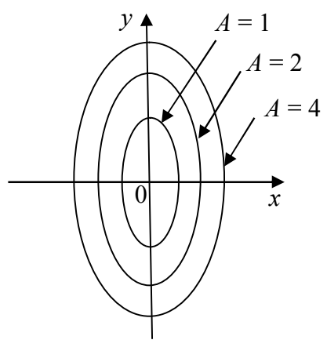
\includegraphics[width=0.3\linewidth]{images/family-soln.png}
\end{figure}
\end{solution}

\subsection{Reduction to separable form by substitution}
Some first order differential equations can be transformed by a suitable substitution into separable form.

\begin{exercise}
Find the general solution of
\[ \dv{y}{x} = \sin(x+y+1) \]
\end{exercise}

\begin{proof}[Solution]
Let $u(x) = x + y(x) + 1$ so that $\dv{u}{x} = 1 + \dv{y}{x}$. Then the original equation can be written as $\dv{u}{x} = 1 + \sin u$, which is separable. We have
\[ \frac{1}{1+\sin u}\dv{u}{x} = 1 \]
which integrates to
\[ \int \frac{1}{1+\sin u} \dd{u} = x+c \]
Let us evaluate the integral on the left hand side:
\begin{align*}
\int \frac{1}{1+\sin u} \dd{u}
&= \int \frac{1-\sin u}{(1+\sin u)(1-\sin u)} \dd{u} \\
&= \int \frac{1-\sin u}{1-\sin^2u} \dd{u} = \int \frac{1-\sin u}{\cos^2u} \dd{u} \\
&= \int \frac{1}{\cos^2u} \dd{u} - \int \frac{\sin u}{\cos^2u} \dd{u} \\
&= \tan u - \frac{1}{\cos u} + c
\end{align*}
Therefore 
\[ \tan u - \frac{1}{\cos u} = x+c \]
In terms of $x$ and $y$, the solution is given by
\[ \tan (x+y+1) - \frac{1}{\cos (x+y+1)} = x+c \]
or
\[ \sin (x+y+1) - 1 = (x+c) \cos (x+y+1). \]
This solution, where we have not found $y$ in terms of $x$, is called an \textbf{implicit solution}.
\end{proof}

A special group of first order differential equations is those of the form
\[ \dv{y}{x} = f\brac{\frac{y}{x}} \]
These differential equations are called \textbf{homogeneous} and they can be solved with a substitution
of the form
\[ y(x) = xv(x) \]
to get a new equation in terms of x and the new dependent variable $v$. This new equation will be
separable:
\[ \dv{y}{x} = v + x\dv{v}{x} \]
which becomes
\[ x\dv{v}{x} = f(v) - v \]

\subsection{Exact solutions}
LHS is an exact derivative.
\begin{exercise}
Solve 
\[ \sin x\dv{y}{x}+y\cos x=3x^2. \]
\end{exercise}
\begin{proof}[Solution]
Notice that the LHS is an exact derivative.
\begin{align*}
\sin x\dv{y}{x}+y\cos x &= \dv{x}y\sin x \\
\dv{x}y\sin x &= 3x^2 \\
y \sin x &= \int 3x^2\dd{x} = x^3+c \\
y &= \frac{x^3+c}{\sin x}
\end{align*}
\end{proof}

\subsection{Integrating Factor}
Looking specifically at first order linear ODEs, which take the general form
\[ \dv{y}{x} + P(x)y = Q(x) \]
we see that the homogeneous form, that is when $Q(x)=0$, is separable. On the other hand, the inhomogeneous form can be solved using an \textbf{integrating factor} $I(x)$ given by
\[ I(x) = e^{\int P(x) \dd{x}} \]
\begin{proof}
Simply multiply the general equation for first-order linear ODEs through by the integrating factor to obtain
\[ e^{\int P(x) \dd{x}} \dv{y}{x} + P(x) e^{\int P(x) \dd{x}}y = e^{\int P(x) \dd{x}} Q(x) \]
Using the product rule for derivatives, we see that this gives
\[ \dv{}{x}\brac{e^{\int P(x) \dd{x}}y} = e^{\int P(x) \dd{x}} Q(x) \]
and we can now integrate directly and rearrange, to obtain
\[ y = e^{-\int P(x) \dd{x}} \sqbrac{\int e^{\int P(x)dx} Q(x) \dd{x} + c}. \]
\end{proof}

\begin{exercise}
Solve the linear differential equation 
\[ \dv{y}{x} + 2xy = 2xe^{-x^2}. \]
\end{exercise}
\begin{solution}
We can easily see that the given differential equation is in the form of a first-order linear ODE.

First we find the integrating factor:
\[ I(x) = e^{\int 2x \dd{x}} = e^{x^2} \]

Multiplying the given differential equation through by the integrating factor this gives
\[ e^{x^2} \dv{y}{x} + 2xe^{x^2}y = 2x \]
that is
\[ \dv{}{x}\brac{e^{x^2}y}= 2x \]
Integrating this gives us
\[ e^{x^2}y = x^2 + c \]
so the general solution is $y = (x^2+c)e^{-x^2}$.
\end{solution}

\subsection{Qualitative approach}
\subsubsection{Slope field}


\subsubsection{Bifurcation diagram}

\subsection{Numerical methods}
\subsubsection{Euler's method}
The key principle in Euler's method is the use of a linear approximation for the tangent line to the actual solution curve $y(t)$ to approximate a solution.

Given an initial value problem
\[ \dv{y}{t}=f(t,y), \quad y(t_0)=y_0, \]
we start at $(t_0,y_0)$ on the solution curve as shown in the figure below. The equation of the tangent line through $(t_0,y_0)$ is given by
\begin{align*}
\frac{y-y_0}{t-t_0}&=f(t_0,y_0)\\
y-y_0&=(t-t_0)f(t_0,y_0)\\
y&=y_0+(t-t_0)f(t_0,y_0)
\end{align*}

\begin{figure}[H]
    \centering
    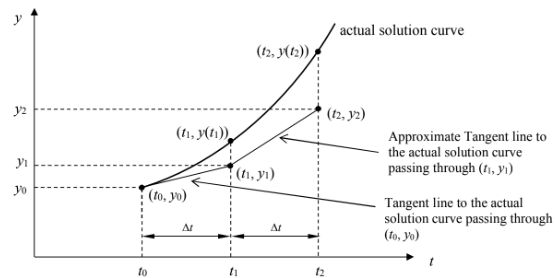
\includegraphics[width=0.75\linewidth]{images/euler-method-de.png}
\end{figure}

If we choose a step size of $\Delta t$ on the $t$-axis, then $t_1=t_0+\Delta t$. By using Euler's method, at $t=t_1$, we can obtain an approximate value $y_1$ from
\[ y_1=y_0+(t_1-t_0)f(t_0,y_0). \]
The point $(t_1,y_1)$ on the tangent line is an approximation to the point $(t_1,y(t_1))$ on the actual solution curve; that is, $y_1\approx y(t_1)$. From the figure, it is observed that the accuracy of the approximation depends heavily on the size of $\Delta t$. Hence we must choose an increment $\Delta t$ which is ``reasonably small''.

At $t=t_2$, we can similarly find the approximate valye $y_2$ from
\[ y_2=y_1+(t_2-t_1)f(t_1,y_1). \]
In general, at $t=t_{n+1}$, it follows that
\[ y_{n+1}=y_n+(t_{n+1}-t_n)f(t_n,y_n). \]
Substituting $\Delta t=t_{n+1}-t_n$, we have Euler's formula as follows:
\begin{equation}
y_{n+1}=y_n+\Delta t\cdot f(t_n,y_n)
\end{equation}
for $n=0,1,2,\dots$

\subsubsection{Improved Euler's method}
The improved Euler's method works as follows: We first apply Euler's method to find an approximation to an intermediate $y$ value and denote it as $\bar{y}_{n+1}$. We then apply Euler's method again, but now we use a linear line segment whose slope is the average of $f(t_n,y_n)$ and $f(t_{n+1},\bar{y}_{n+1})$.

\begin{figure}[H]
    \centering
    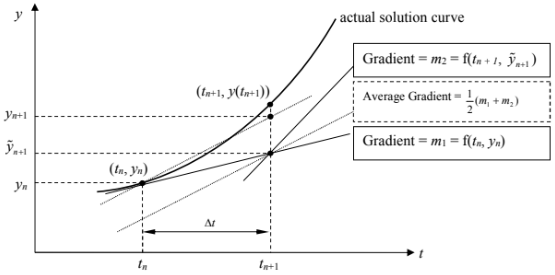
\includegraphics[width=0.75\linewidth]{images/euler-method-de-improved.png}
\end{figure}

The Improved Euler's method (also known as the Heun’s formula) consists of two steps:
\begin{equation}
\begin{split}
\bar{y}_{n+1}&=y_n+\Delta t\cdot f(t_n,y_n)\\
y_{n+1}&=y_n+\Delta t\cdot\sqbrac{\frac{f(t_n,y_n)+f(t_{n+1},\bar{y}_{n+1})}{2}}
\end{split}
\end{equation}
\pagebreak

\section{Second-order homogeneous linear ODEs}
This section introduces a method for finding a second solution to a second order homogeneous linear ODE, when one solution has already been found. Suppose $z(x)\neq0$ is a non-trivial solution to the second order homogeneous linear differential equation
\[ P(x)\dv[2]{y}{x}+Q(x)\dv{y}{x}+R(x)y=0. \]
We can make the substitution $y(x)=u(x)z(x)$, so that
\[ \dv{y}{x}=\dv{u}{x}z+u\dv{z}{x} \quad \text{and} \quad \dv[2]{y}{x}=\dv[2]{u}{x}z+2\dv{u}{x}\dv{z}{x}+u\dv[2]{z}{x}. \]
Substituting these into the above equation and using the prime to denote the derivative with respect to $x$ we obtain
\[ P(x)\brac{u^{\prime\prime}z+2u^\prime z^\prime+uz^{\prime\prime}}+Q(x)\brac{u^\prime z+uz^\prime}+R(x)uz=0. \]
If we now rearrange the above equation and use the fact that $z$ is a solution to the given equation then we get
\[ P(x)zu^{\prime\prime}+\brac{2P(x)z^\prime+Q(x)z}u^\prime=0, \]
which is a homogeneous differential equation of first order for $u^\prime$. In theory this can be solved, to obtain the general solution to the given equation. The following example illustrates this technique.

\begin{exercise}
Verify that $z(x)=\frac{1}{x}$ is a solution to
\[ x\dv[2]{y}{x}+2(1-x)\dv{y}{x}-2y=0, \]
and hence find its general solution.
\end{exercise}
\begin{solution}

\end{solution}


\todo{To edit}
\subsection{Linear with constant coefficients}
For equations in the form 
\[ a\dv[2]{y}{x} + b\dv{y}{x} +cy = 0 \]
we can write out the \textbf{auxiliary equation}
\[ am^2+bm+c=0 \]
which has roots
\[ m_{1,2}=\frac{-b\pm \sqrt{b^2-4ac}}{2a}. \]

From the nature of the roots of the auxiliary equation, we can deduce the corresponding type of general solution.
\begin{table}[H]
\centering
\begin{tabular}{c|c}
\hline\hline
\textbf{Roots of auxiliary equation} & \textbf{General solution} \\
\hline
real and distinct & $y=Ae^{m_1x}+Be^{m_2x}$ \\
real and repeated & $y=e^{mx}(A+Bx)$ \\
imaginary: $m=\alpha\pm i\beta$ & $y=e^{\alpha x}(A\cos\beta x+B\sin\beta x)$ \\
\hline\hline
\end{tabular}
\end{table}

\subsection{Non-linear}
Equation
\[ a\dv[2]{y}{x} + b\dv{y}{x} +cy = f(x) \]
where $a\neq0$, $f(x)\neq0$

General solution y=Complementary Function (CF)+Particular Integral (PI)
Complementary function: solution of the homogeneous equation

Particular integral (PI)
find by seeing different cases of f(x) and then y,dy/dx,d2y/dx2 of general PI into DE to find unknown constants of PI
If f(x) is a polynomial of degree n, $y=a_nx^n+a_{n-1}x^{n-1}+\cdots+a_1x+a_0$
When DE is a*d2y/dx2+b*dy/dx=f(x),
method 1: find CF and let PI be
\[ y=x(a_nx^n+a_{n-1}x^{n-1}+\cdots+a_1x+a_0) \]
method 2: integrate both sides wrt x and then solve accordingly

If $f(x)=qe^{kx}$ where $k$ and $q$ are constants, 

If $f(x)=k\cos ax$ or $f(x)=k\sin ax$ or $f(x)=k\cos ax+k\sin ax$

If $f(x)$ is the sum of various functions

\begin{example}[Vibrating springs]
Restoring force is given by $F=-kx$. By Newton's 2nd Law, we have $m\dv[2]{x}{t}=-kx$, or
\[ m\dv[2]{x}{t}+kx=0. \]
Hence we have auxilliary equation $mr^2+k=0$ with roots $r=\pm\omega i$ where angular frequency $\omega=\sqrt{\frac{k}{m}}$.

Thus the general solution is
\[ x(t)=c_1\cos\omega t+c_1\sin\omega t. \]
Using R-formula,
\[ x(t)=R\cos(\omega t+\delta) \]
where amplitude $R=\sqrt{c_1^2+c_2^2}$, $\cos\delta=\frac{c_1}{R}$, $\sin\delta=-\frac{c_2}{R}$, $\delta$ is known as phase angle. Period $T=\frac{2\pi}{\omega}=2\pi\sqrt{\frac{m}{k}}$.
\end{example}

\begin{example}[Damping vibrations]
Damping force is given by $F=-c\dv{x}{t}$. By Newton's 2nd law, $m\dv[2]{x}{t}=-kx-c\dv{x}{t}$, or
\[ m\dv[2]{x}{t}+c\dv{x}{t}+kx=0 \]
which has auxilliary equation $mr^2+cr+k=0$.
\begin{itemize}
\item Case 1: $c^2-4mk>0$ (over-damping)

Solution is
\[ x=c_1e^{r_1t}+c_2e^{r_2t}. \]

\item Case 2: $c^2-4mk=0$ (critical damping)

Solution is
\[ x=(c_1+c_2)e^{rt}. \]

\item Case 3: $c^2-4mk<0$ (under-damping)

Roots of auxilliary equation are $r=-\frac{c}{2m}\pm\omega i$ where $\omega=\frac{\sqrt{4mk-c^2}}{2m}$.

Solution is
\[ x=e^{-\frac{c}{2m}t}(c_1\cos\omega t+c_2\sin\omega t). \]

Amplitude follows the graph
\[ x=\pm Ae^{-\frac{c}{2m}t} \]
where $A=\sqrt{c_1^2+c_2^2}$.

For damped forced vibrations,
\[ m\dv[2]{x}{t}+c\dv{x}{t}+kx=F(t) \]
where $F(t)$ is external force.
\end{itemize}

\end{example}

\begin{example}[Electric circuits]
\[ L\dv{I}{t}+RI+\frac{Q}{C}=E \]
where $L$ is inductance, $R$ is resistance, $C$ is capacitance, $Q$ is charge, $I=\dv{Q}{t}$ is current, $E(t)$ is e.m.f.

Rewriting and taking time derivative,
\[ L\dv[2]{I}{t}+R\dv{I}{t}+\frac{1}{C}I=E^\prime(t). \]
\end{example}



Population Dynamics and Population Growth Models\todo{To look for info from F Maths notes}
• exponential growth model
• logistic growth model, equilibrium points and
their stability, and harvesting

\section{Laplace Transforms}
\subsection{Definition}
\begin{definition}
Suppose that $f(t)$ is a piecewise continuous function. The Laplace transform of $f(t)$ is denoted $\mathcal{L}\{f(t)\}$ and defined as
\begin{equation}
\mathcal{L}\{f(t)\}=\int_0^\infty e^{-st}f(t)\dd{t}.
\end{equation}
\end{definition}

\begin{notation}
For the sake of convenience we will often denote Laplace transforms as
\[ \mathcal{L}\{{f(t)}\}=F(s). \]
\end{notation}

\section{Systems of Differential Equations}
\pagebreak

\part{Calculus (Multivariable)}
\chapter{Partial Derivatives}
In multivariable calculus, we extend notions of differential calculus from functions of one variable to more general functions
\[ f:\RR^n\to\RR^m. \]

\section{Computation of partial derivatives}
Let $f:\RR^n\to\RR$ be a function of $n$ variables $x_1,x_2,\dots,x_n$. Then the \vocab{partial derivative}
\[ \pdv{f}{x_i}(p_1,\dots,p_n) \]
is the rate of change of $f$, at $(p_1,\dots,p_n)$, when we vary only the variable $x_i$ about $p_i$ and keep all of the other variables constant. Precisely, we have
\begin{equation}\label{eqn:partial-diff}
\pdv{f}{x_i}(p_1,\dots,p_n)=\lim_{h\to0}\frac{f(p_1,\dots,p_{i-1},p_i+h,p_{i+1},\dots,p_n)-f(p_1,\dots,p_n)}{h}.
\end{equation}

\begin{notation}
We shall occasionally write $f_x$ for $\delta f/\delta x$, etc.
\end{notation}

Derivatives such as \cref{eqn:partial-diff}, where $f$ has been differentiated once, are called \vocab{first order} partial derivatives. We will look at higher orders in a moment.

\begin{exercise}
Find all the first order derivatives of
\[ f(x,y,z)=x^2+ye^{2x}+\frac{z}{y}. \]
\end{exercise}

\begin{solution}
Keep in mind that we only need to find the derivative of functions with respect to one variable by keeping the rest of the variables constant.

Thus we have
\[ \pdv{f}{x}=2x+2ye^{2x}, \quad \pdv{f}{y}=e^{2x}-\frac{z}{y^2}, \quad \pdv{f}{z}=\frac{1}{y}. \]
\end{solution}

We define second and higher order partial derivatives in a similar manner to how we define them for full derivatives. So, in the case of second order partial derivatives of a function $f(x,y)$ we have
\[ \begin{split}
f_{xx} &= \pdv{}{x}\brac{\pdv{f}{x}} = \pdv[order={2}]{f}{x} \\
f_{yy} &= \pdv{}{y}\brac{\pdv{f}{y}} = \pdv[order={2}]{f}{y} \\
f_{xy} &= \pdv{}{y}\brac{\pdv{f}{x}} = \pdv{f}{x,y} \\
f_{yx} &= \pdv{}{x}\brac{\pdv{f}{y}} = \pdv{f}{y,x}
\end{split} \]

Observe that
\[ \pdv{f}{y,x}=\pdv{f}{x,y}, \quad \pdv{f}{z,x}=\pdv{f}{x,z}, \quad \pdv{f}{z,y}=\pdv{f}{y,z}. \]
This will typically be the case in the examples we will see in this course, but it is not guaranteed unless the derivatives in question are continuous.

we might have a function $f(u,v)$ of two variables $u$ and $v$, each of which is itself a function of $x$ and $y$. We can make the composition
\[ F(x,y)=f(u(x,y),v(x,y)) \]
which is a function of $x$ and $y$, and we might then want to calculate the partial derivatives
\[ \pdv{F}{x}\text{ and }\pdv{F}{y}. \]

\begin{theorem}[Chain rule]
Let $F(t)=f(u(t),v(t))$ with $u$ and $v$ differentiable and $f$ being continuously differentiable in each variable. Then
\begin{equation}
\dv{F}{t}=\pdv{f}{u}\pdv{u}{t}+\pdv{f}{v}\pdv{v}{t}
\end{equation}
\end{theorem}

\begin{corollary}
Let $F(x,y)=f(u(x,y),v(x,y))$ with $u$ and $v$ differentiable in each variable and $f$ being continuously differentiable in each variable. Then
\[ \pdv{F}{x}=\pdv{f}{u}\pdv{u}{x}+\pdv{f}{v}\pdv{v}{x}, \quad \pdv{F}{y}=\pdv{f}{u}\pdv{u}{y}+\pdv{f}{v}\pdv{v}{y}. \]
\end{corollary}

\begin{exercise}
A particle $P$ moves in three dimensional space on a helix so that at time $t$,
\[ x(t)=\cos t, \quad y(t)=\sin t, \quad z(t)=t. \]
The temperature $T$ at $(x,y,z)$ equals $xy+yz+zx$. Use the chain rule to calculate $\dv{T}{t}$.
\end{exercise}

\begin{solution}
The chain rule in this case says that
\begin{align*}
\dv{T}{t} &= \pdv{T}{x}\dv{x}{t}+\pdv{T}{y}\dv{y}{t}+\pdv{T}{z}\dv{z}{t} \\
&= (y+z)(-\sin t)+(x+z)\cos t+(y+x)(1) \\
&= (\sin t+t)(-\sin t)+(\cos t+t)\cos t+(\cos t+\sin t) \\
&= -\sin^2t+\cos^2t+\sin t+\cos t+t\cos t-t\sin t.
\end{align*}
\end{solution}

\begin{exercise}
Let $z=f(xy)$, where $f$ is an arbitrary differentiable function in one variable. Show that
\[ x\pdv{z}{x}-y\pdv{z}{y}=0. \]
\end{exercise}

\begin{solution}
By the chain rule,
\[ \pdv{z}{x}=yf^\prime(xy) \quad \text{and} \quad \pdv{z}{y}=xf^\prime(xy), \]
where the prime denotes the derivative with respect to $xy$. Hence we have
\[ x\pdv{z}{x}-y\pdv{z}{y}=xyf^\prime(xy)-yxf^\prime(xy)=0. \]
\end{solution}

\section{Directional Derivatives}
To this point we've only looked at the two partial derivatives $f_x(x,y)$ and $f_y(x,y)$. Recall that these derivatives represent the rate of change of $f$ as we vary x (holding $y$ fixed) and as we vary $y$ (holding $x$ fixed) respectively. 

We now discuss how to find the rate of change of $f$ if we allow both $x$ and $y$ to change simultaneously. The problem here is that there are many ways to allow both $x$ and $y$ to change. For instance, one could be changing faster than the other and then there is also the issue of whether or not each is increasing or decreasing. So, before we get into finding the rate of change we need to get a couple of preliminary ideas taken care of first. The main idea that we need to look at is just how are we going to define the changing of $x$ and/or $y$.

Let's start off by supposing that we wanted the rate of change of $f$ at a particular point, say $(x_0,y_0)$. Let's also suppose that both $x$ and $y$ are increasing and that, in this case, $x$ is increasing twice as fast as $y$ is increasing. So as $y$ increases one unit of measure, $x$ increases two units of measure.

Let's suppose that a particle is sitting at $(x_0,y_0)$ and the particle will move in the direction given by the changing 
$x$ and $y$. At this point, the particle can be said to be moving in the direction
\[ \vec{v} = \langle {2,1} \rangle \]

There is still a small problem with this however. There are many vectors that point in the same direction. For instance, all of the following vectors point in the same direction as $\vec v = \langle {2,1} \rangle$:
\[ \vec{v} = \left\langle {\frac{1}{5},\frac{1}{10}}\right\rangle \quad \vec{v} = \langle {6,3}\rangle \quad \vec{v} = \left\langle {\frac{2}{\sqrt{5}},\frac{1}{\sqrt{5}}}\right\rangle \]

We need a way to consistently find the rate of change of a function in a given direction. We will do this by insisting that the vector that defines the direction of change be a unit vector. This means that for the example that we started off thinking about we would want to use
\[ \vec{v} = \left\langle {\frac{2}{\sqrt{5}},\frac{1}{\sqrt{5}}}\right\rangle \]

\begin{definition}[Directional derivative]
Rate of change of $f(x,y)$ in the direction of the unit vector $\vec{u}=\langle{a,b}\rangle$ is called the directional derivative and is denoted by $D_{\vec{u}} f(x,y)$.

The definition of the directional derivative is
\begin{equation}
{D_{\vec u}}f(x,y) = \lim_{h\to0} \frac{f(x + ah,y + bh) - f(x,y)}{h}
\end{equation}
\end{definition}

To derive an equivalent formula for taking directional derivatives, we define a new function of a single variable
\[ g(z) = f(x_0+az,y_0+bz) \]
where $x_0$, $y_0$, $a$, $b$ are some fixed numbers. Note that this really is a function of a single variable $z$.

Then by the definition of the derivative for functions of a single variable we have
\[ g^\prime(z) = \lim_{h\to0} \frac{g(z+h)-g(z)}{h} \]
and the derivative at $z=0$ is given by
\[ g^\prime(0) = \lim_{h\to0} \frac{g(h)-g(0)}{h} \]
If we now substitute in for $g(z)$ we get
\[ g^\prime(0) = \lim_{h\to0} \frac{g(h)-g(0)}{h} = \lim_{h\to0} \frac{f(x_0+ah,y_0+bh) - f(x_0,y_0)}{h} = D_{\vec u}f(x_0,y_0) \]
This gives us
\begin{equation}\tag{1}
g^\prime(0) = D_{\vec u}f(x_0,y_0)
\end{equation}

Now, let's look at this from another perspective. Let's rewrite $g(z)$ as $g(z) = f(x,y)$ where $x=x_0+az$ and $y=y_0+bz$. Applying chain rule,
\[ g^\prime(z) = \odv{g}{z} = \pdv{f}{x}\odv{x}{z} + \pdv{f}{y}\odv{y}{z} = f_x (x,y)a + f_y (x,y)b \]
This gives us
\[ g^\prime(z) = f_x (x,y)a + f_y (x,y)b \]
If we take $z=0$ we get $x=x_0$ and $y=y_0$. Plugging these into the above equation gives
\begin{equation}\tag{2}
g^\prime(0) = f_x (x_0,y_0)a + f_y (x_0,y_0)b
\end{equation}
Equating (1) and (2) gives
\[ {D_{\vec u}}f(x_0,y_0) = f_x(x_0,y_0)a + f_y(x_0,y_0)b \]
Allowing $x$ and $y$ to be any number we get the following formula for computing directional derivatives:
\[ {D_{\vec u}}f(x,y) = f_x(x,y)a + f_y(x,y)b \]
For three variables, directional derivative of $f(x,y,z)$ in the direction of the unit vector $\vec{u}=\langle{a,b,c}\rangle$ is given by
\begin{equation}
{D_{\vec u}}f(x,y,z) = f_x (x,y,z)a + f_y (x,y,z)b + f_z (x,y,z)c
\end{equation}

We can write the directional derivative as a \textbf{dot product} and notice that the second vector is nothing more than the unit vector $\vec u$ that gives the direction of change.
\begin{equation}
{D_{\vec u}} f(x,y,z) = \langle {f_x,f_y,f_z} \rangle \cdot \langle {a,b,c} \rangle
\end{equation}

Now let's give a name and notation to the first vector in the dot product since this vector will show up fairly regularly.
\begin{definition}[Gradient vector]
The gradient vector of $f$ is defined to be
\begin{equation}
\nabla f = \langle f_x,f_y,f_z \rangle
\end{equation}
\end{definition}

With the definition of the gradient we can now say that the directional derivative is given by
\[ {D_{\vec u}}f = \nabla f\cdot \vec u \]

\begin{theorem}
Maximum value of $D_{\vec u} f(\vec{x})$ (and hence then the maximum rate of change of the function $f(\vec{x})$) is given by $\left\|\nabla f(\vec{x})\right\|$ and will occur in the direction given by $\nabla f(\vec{x})$.
\end{theorem}

\begin{proof}

\end{proof}
\pagebreak

\chapter{Partial Differential Equations}
\section{Definitions and Terminology}
\begin{definition}
A \vocab{partial differential equation} is an equation involving a function and/or its partial derivatives. 
\end{definition}

We can classify PDEs based on:
\begin{itemize}
\item \textbf{Order.}

The order is the number corresponding to the order of the highest partial derivative in the equation. 

For instance, the order of the following PDE is 2. 
\[ \pdv[order={2}]{f}{x}=\pdv{f}{t} \]

This also applies to mixed partial derivatives. For instance, the order of the following PDE is 3.
\[ \pdv[order={2,1}]{f}{x,y}=\pdv{f}{t} \]

\item \textbf{Number of independent variables.}

An independent variable is what we differentiate with respect to. 

\item \textbf{Linearity.}

A linear PDE is one in which the \emph{dependent} variable (the one being differentiated) appears only in a linear fashion.

For instance, the two PDEs above are linear as the partial derivatives are not being raised to a power or multiplied with each other.

The following PDE is non-linear.
\[ f\pdv[order={2}]{f}{x}=\pdv{f}{t} \]

\item \textbf{Homogeneity.}

A homogenous PDE is one in which every term only involves the dependent variable and/or its derivatives.

The first two PDEs above are homogenous as every term contains $f$ or its derivatives.

The following PDE is non-homogenous as there are two terms that do not contain $f$.
\[ \pdv[order={2}]{f}{x}=\pdv{f}{t}+x^2+\tan t \]

\item \textbf{Coefficient type.}

The coefficient here refers to the coefficient of the term involving the dependent variable and its derivatives. It can be either constant or variable.

For instance, the coefficients of the terms in the first two examples are 1. We say that these two PDEs have constant coefficients.

The following PDE has variable coefficients.
\[ \tan x\pdv[order={2}]{f}{x}=\pdv{f}{t} \]

\item \textbf{Parabolic, Hyperbolic, or Elliptic.}

We can do this classification for linear 2nd order PDEs which take the form of 
\[ A\pdv[order={2}]{f}{x} + B\pdv{f}{x,y} + C\pdv[order={2}]{f}{y} + D\pdv{f}{x} + E\pdv{f}{y} + Ff = G \]
where the coefficients are generally functions of $x$ or $y$.

For a \textbf{hyperbolic} PDE, $B^2-4AC>0$. Using variable substitutions to change $x$ and $y$ to $\eta$ and $\epsilon$ respectively, we can reduce the PDE to \[ \pdv[order={2}]{f}{\eta} - \pdv[order={2}]{f}{\epsilon} + g = 0 \] where $g$ denotes the first and lower order terms. This is similar to the equation of a hyperbola: $x^2-y^2=1$.

For a \textbf{parabolic} PDE, $B^2-4AC=0$. Using variable substitutions, we can reduce the PDE to \[ \pdv[order={2}]{f}{\eta} + g = 0. \] This is similar to the equation of a parabola: $x^2+y=0$.

For an \textbf{elliptic} PDE, $B^2-4AC<0$. Using variable substitutions, we can reduce the PDE to \[ \pdv[order={2}]{f}{\eta} + \pdv[order={2}]{f}{\epsilon} + g = 0. \] This is similar to the equation of an ellipse: $x^2+y^2=1$.

Note that if the coefficients are constants, the PDE can be hyperbolic, parabolic or elliptic. However, if the coefficients are variables, then it is possible for the PDE to be hyperbolic in some regions, and elliptic or parabolic in some regions.
\end{itemize}

\section{Solutions and Auxiliary Conditions}
\begin{exercise}
Show that $f(x,y)=\tan^{-1}\frac{y}{x}$ satisfies Laplace's equation in the plane:
\[ \pdv{[order={2}]}{f}{x}+\pdv{[order={2}]}{f}{y}=0. \]
\end{exercise}

\begin{solution}
The first order partial derivatives are
\[ \pdv{f}{x}=\frac{1}{1+\brac{\frac{y}{x}}^2}\brac{-\frac{y}{x^2}}=-\frac{y}{x^2+y^2} \]
and
\[ \pdv{f}{y}=\frac{1}{1+\brac{\frac{y}{x}}^2}\brac{\frac{1}{x}}=\frac{x}{x^2+y^2}. \]
Hence we have
\[ \pdv{[order={2}]}{f}{x}=\frac{2xy}{x^2+y^2} \quad \text{and} \quad \pdv{[order={2}]}{f}{y}=-\frac{2xy}{(x^2+y^2)^2}, \]
from which we see that
\[ \pdv{[order={2}]}{f}{x}+\pdv{[order={2}]}{f}{y}=0 \]
as required.
\end{solution}

In the above example we verified that a given solution satisfied a given PDE. We now look at how to find solutions to simple PDEs.

\begin{exercise}
Find all the solutions of the form $f(x,y)$ of the PDEs
\begin{enumerate}[label=(\alph*)]
\item $\pdv{f}{y,x}=0$,
\item $\pdv{[order={2}]}{f}{x}=0$.
\end{enumerate}
\end{exercise}

\begin{solution} \
\begin{enumerate}[label=(\alph*)]
\item We have
\[ \pdv{}{y}\brac{\pdv{f}{x}}=0. \]
Those functions $g(x,y)$  which satisfy $\delta g/\delta y=0$ are functions which solely depend on $x$. So we have
\[ \pdv{f}{x}=p(x), \]
where $p$ is an arbitrary function of $x$. We can now integrate again, but this time with respect to $x$ rather than $y$. Now, $\delta/\delta x$ sends to zero any function which solely depends on $y$. The solution to the PDE is therefore
\[ f(x,y)=P(x)+Q(y), \]
where $Q(y)$ is an arbitrary function of $y$ and $P(x)$ is an anti-derivative of $p(x)$, i.e. $P^\prime(x)=p(x)$.
\end{enumerate}
\end{solution}

If a PDE involves derivatives with respect to one variable only, we can treat it like an ODE in that variable, holding all other variables constant. The difference, as noted above, is that our arbitrary ``constants'' will now be arbitrary functions of the variables that we have held constant.

\begin{exercise}
Find solutions $u(x,y)$ of the PDE
\[ u_{xx}-u=0. \]
\end{exercise}

\begin{solution}
Since there are no derivatives with respect to $y$, we can solve the associated ODE
\[ \dv[2]{u}{x}-u=0, \]
where $u$ is treated as being a function of $x$ only. This ODE has solution $u(x)=C_1e^x+C_2e^{-x}$, where $C_1$ and $C_2$ are constants, and so the solution to the original PDE is
\[ u(x,y)=A(y)e^x+B(y)e^{-x}, \]
where $A$ and $B$ are arbitrary functions of $y$ only.
\end{solution}

we look at one specific method for solving PDEs, that of \textbf{separating the variables}.

\begin{exercise}
Find all solutions of the form $T(x,t)=A(x)B(t)$ to the one-dimensional heat/diffusion equation
\[ \pdv{T}{t}=\kappa\pdv{[order={2}]}{T}{x}, \]
where $\kappa$ is a positive constant, called the thermal diffusivity.
\end{exercise}

Solutions of the form $A(x)B(t)$ are known as separable solutions

There are a lot of solutions to a given PDE, hence it is important for us to know the auxiliary conditions, i.e. boundary and initial conditions, which dictate which technique we use to solve the PDE.
\begin{itemize}
\item A boundary condition expresses the behavior of a function on the boundary (border) of its area of definition. An initial condition is like a boundary condition, but then for the time-direction.
\end{itemize}
\pagebreak

\chapter{Multiple Integrals}
\section{Double Integrals}
To motivate the idea of double integrals, we give an example of calculating areas.

We want to integrate a function of two variables, $f(x,y)$. With functions of one variable we integrated over an \emph{interval} (i.e. a one-dimensional space) and so it makes some sense then that when integrating a function of two variables we will integrate over a \emph{region} of $\RR^2$ (two-dimensional space). 

\begin{exercise}
Calculate the area of the disc $x^2+y^2\le a^2$.
\end{exercise}

\begin{solution}
we know the answer, namely $\pi a^2$. If we wish to capture all of the disc's area then we let $x$ vary from $-a$ to $a$ and, at each $x$ we let $y$ vary from $-\sqrt{a^2-x^2}$ to $\sqrt{a^2-x^2}$.

Thus we have
\begin{align*}
A &= \int_{x=-a}^{x=a}\int_{y=-\sqrt{a^2-x^2}}^{y=\sqrt{a^2-x^2}}\dd{y}\dd{x} \\
&= \int_{x=-a}^{x=a}2\sqrt{a^2-x^2}\dd{x} \\
&= \int_{\theta=-\frac{\pi}{2}}^{\theta=\frac{\pi}{2}}2\sqrt{a^2-a^2\sin^2\theta}a\cos\theta\dd{\theta} \quad [x=a\sin\theta] \\
&= a^2\int_{\theta=-\frac{\pi}{2}}^{\theta=\frac{\pi}{2}}2\cos^2\theta\dd{\theta}=\pi a^2
\end{align*}
\end{solution}

\begin{definition}
Let $R\subset\RR^2$. Then we define the \vocab{area} of $R$ to be
\[ A(R)=\iint_{(x,y)\in R}\dd{x}\dd{y}. \]
\end{definition}

% https://tutorial.math.lamar.edu/classes/calciii/DoubleIntegrals.aspx

Recall that given a function $f(x)$, the definite integral $\int_a^bf(x)\dd{x}$ evaluates the area under the curve $y=f(x)$ between $x=a$ and $x=b$. Similarly given a function $f(x,y)$, the volume of the solid below the graph $z=f(x,y)$ and above the region $R$ in the $xy$-plane is given by 
\begin{equation}
V=\iint_Rf(x,y)\dd{A}.
\end{equation}

\begin{remark}
You can think of $\iint$ as a sum of heights $f(x,y)$ and areas $\dd{A}$, which evaluates to give a volume.
\end{remark}

\begin{exercise}
Let $R$ be the triangle whose vertices are $(0,0,0)$, $(0,1,0)$ and $(1,0,0)$. Evaluate $\iint_R1\dd{A}$.
\end{exercise}

\begin{solution}
$\iint_R1\dd{A}$ is the volume of a prism with height $1$ and base of area $R$. Hence
\[ \iint_R1\dd{A}=\text{Area of }R\times1=\frac{1}{2}\times1\times1\times1=\boxed{\frac{1}{2}} \]
\end{solution}

To evaluate double integrals we need a notion called iterated integrals, which are basically two integrals with one nested inside the other.

\begin{exercise}
Evaluate 
\begin{enumerate}[label=(\alph*)]
\item $\displaystyle\int_0^1\int_1^2x+2y\dd{x}\dd{y}$
\item $\displaystyle\int_{-1}^1\int_0^x3x^2+2y\dd{y}\dd{x}$
\end{enumerate}
\end{exercise}

\begin{solution}
\begin{enumerate}[label=(\alph*)]
\item 
\begin{align*}
\int_0^1\int_1^2x+2y\dd{x}\dd{y}
&= \int_0^1\brac{\int_1^2x+2y\dd{x}}\dd{y} \\
&= \int_0^1\sqbrac{\frac{x^2}{2}+2yx}_{x=1}^{x=2}\dd{y} \\
&= \int_0^12y+\frac{3}{2}\dd{y} \\
&= \sqbrac{y^2+\frac{3}{2}y}_{y=0}^{y=1}=\boxed{\frac{5}{2}}
\end{align*}

\item 
\begin{align*}
\int_{-1}^1\int_0^x3x^2+2y\dd{y}\dd{x}
&= \int_{-1}^1\brac{\int_0^x3x^2+2y\dd{y}}\dd{x} \\
&= \int_{-1}^1\sqbrac{3x^2y+y^2}_{y=0}^{y=x}\dd{x} \\
&= \int_{-1}^13x^3+x^2\dd{x} \\
&= \sqbrac{\frac{3x^4}{4}+\frac{x^3}{3}}_{x=-1}^{x=1}=\boxed{\frac{2}{3}}
\end{align*}
\end{enumerate}
\end{solution}

\section{Iterated Integrals}
Now we are going to discuss the relation between double integrals and iterated integrals.

$R$ is called simple if $R$ is a rectangle given by $a\le x\le b$ and $c\le y\le d$, in which case
\[ \iint_Rf(x,y)\dd{A}=\int_a^b\int_c^df(x,y)\dd{y}\dd{x}=\int_c^d\int_a^bf(x,y)\dd{x}\dd{y}. \]
This is known as Fubini's Theorem.

$R$ is called vertically simple if $R$ is given by $a\le x\le b$, $g(x)\le y\le h(x)$, in which case
\[ \iint_Rf(x,y)\dd{A}=\int_a^b\int_{g(x)}^{h(x)}f(x,y)\dd{y}\dd{x}. \]

$R$ is called horizontally simple if $R$ is given by $c\le y\le d$, $g(y)\le x\le h(y)$, in which case
\[ \iint_Rf(x,y)\dd{A}=\int_c^d\int_{g(y)}^{h(y)}f(x,y)\dd{x}\dd{y}. \]

% https://tutorial.math.lamar.edu/Classes/CalcIII/DIGeneralRegion.aspx
\pagebreak

\chapter{Line Integrals}
\section{Vector fields}
A vector field is basically what you get when associating each point in space with a vector.

\begin{definition}
A \vocab{vector field} on two (or three) dimensional space is a function $\vec{F}$ that assigns eahc point $(x,y)$ (or $(x,y,z)$) a two (or three) dimensional vector given by $\vec{F}(x,y)$ (or $\vec{F}(x,y,z)$).
\end{definition}

The standard notation for the function $\vec{F}$ is:
\begin{align*}
\vec{F}(x,y) &= P(x,y)\hat{i} + Q(x,y)\hat{j} \\
\vec{F}(x,y,z) &= P(x,y,z)\hat{i} + Q(x,y,z)\hat{j} + R(x,y,z)\hat{k}
\end{align*}
depending on whether or not we're in two or three dimensions. The functions $P$, $Q$, $R$ are called \textbf{scalar functions}.

\begin{exercise}
Sketch the following vector field:
\[ \vec{F}(x,y) = -y\hat{i} + x\hat{j} \]
\end{exercise}
\begin{solution}
To graph the vector field we need to get some ``values'' of the function. This means plugging in some points into the function. Here are a couple of evaluations:
\begin{align*}
\vec{F}\brac{{\frac{1}{2},\frac{1}{2}}} &=  -\frac{1}{2}\hat{i} + \frac{1}{2}\hat{j} \\
\vec{F}\brac{{\frac{1}{2},-\frac{1}{2}}} &=  -\brac{{-\frac{1}{2}}}\hat{i} + \frac{1}{2}\hat{j} = \frac{1}{2}\hat{i} + \frac{1}{2}\hat{j} \\
\vec{F}\brac{{\frac{3}{2},\frac{1}{4}}} &=  -\frac{1}{4}\hat{i} + \frac{3}{2}\hat{j}
\end{align*}
So what do these evaluations tell us? The first one tells us that at the point $\brac{\dfrac{1}{2},\dfrac{1}{2}}$ we plot the vector $-\frac{1}{2}\hat{i} + \frac{1}{2}\hat{j}$.

Plotting points gives us the following sketch of the vector field:

\begin{figure}[H]
    \centering
    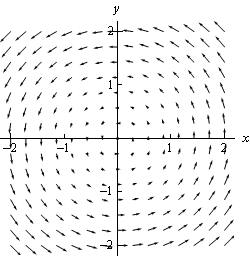
\includegraphics[width=8cm]{images/vec_field2.png}
\end{figure}
\end{solution}

Recall that given a function $f(x,y,z)$ the gradient vector is defined as such:
\begin{definition}
Given a function $f(x,y,z)$, the gradient vector is defined by
\[ \nabla f\coloneqq\left\langle {{f_x},{f_y},{f_z}} \right\rangle. \]
This is a vector field and is often called a \vocab{gradient vector field}.
\end{definition}

\section{Types of line integrals}

\section{Fundamental Theorem for Line Integrals}
\begin{theorem}[Fundamental Theorem of Line Integrals]
Suppose that $C$ is a smooth curve from points $A$ to $B$ parameterised by $\vb{r}(t)$ for $t\in[a,b]$. Let $f$ be a differentiable function whose domain includes $C$ and whose gradient vector $\nabla f$ is continuous on $C$. Then
\begin{equation}
\int_C \nabla f \dd{\vb{r}} = f(\vb{r}(b)) - f(\vb{r}(a)) = f(B) - f(A)
\end{equation}
\end{theorem}

\begin{remark}
Similar to the fundamental theorem of calculus, the primary change is that gradient $\nabla f$ takes the place of the derivative $f^\prime$.
\end{remark}
% https://www.math.uci.edu/~ndonalds/math2e/16-3fundthm.pdf
% https://www.youtube.com/watch?v=_60sKaoRmhU

\section{Conservative Vector Fields}

\section{Green's Theorem}


to compute arc lengths, areas of curves 

applications of integrals to find area and volume

\chapter{Surface Integrals}


\part{Differential Geometry}
\textbf{Readings:}
\begin{itemize}
\item \href{https://aetemad.iut.ac.ir/sites/aetemad.iut.ac.ir/files/files_course/william_m._boothby_an_introduction_to_differentibookfi.org_.pdf}{Introduction to Differentiable Manifolds and Riemannian Geometry}
\item \href{http://www2.ing.unipi.it/griff/files/dC.pdf}{Differential Geometry of Curves and Surfaces}
\end{itemize}